\documentclass{article}
\usepackage{amsmath}
\usepackage{graphicx}
\usepackage{xcolor}
\usepackage{listings}
\usepackage{geometry}
\usepackage{circuitikz}
\geometry{legalpaper, left=20mm,top=25mm}
\usepackage[utf8]{inputenc}
\renewcommand{\familydefault}{\sfdefault}
\renewcommand{\baselinestretch}{1.5}

\definecolor{numberingcolor}{rgb}{1,0,0}
\definecolor{backgroundcolour}{rgb}{0.97,0.97,0.97}

\lstdefinestyle{CodeStyle}{
  backgroundcolor=\color{backgroundcolour},
  numberstyle=\tiny\color{numberingcolor},
  basicstyle=\ttfamily\footnotesize,
  breakatwhitespace=false,         
  breaklines=false,                 
  captionpos=b,                    
  keepspaces=true,                 
  numbers=left,                    
  numbersep=5pt,                  
  showspaces=false,                
  showstringspaces=false,
  showtabs=false,                  
  tabsize=7
}
\lstset{style=CodeStyle}

\title{EE3113 Homework Assignment-1}
\author{Krishna Srikar Durbha}
\date{EE18BTECH11014}

\begin{document}
\maketitle
\vspace{0.1in}
\textbf{Note:} Mathematical Explanations for some of the questions are at the end. 
%% Question-1
\section{Spice Analysis}
\begin{center}
    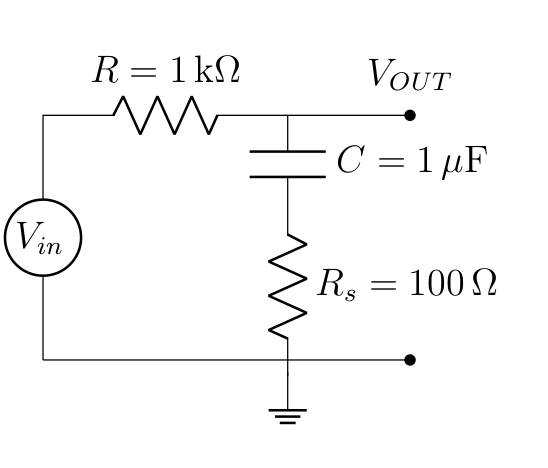
\includegraphics[scale=0.35]{Images/1.png}
\end{center}

% Question-1a
\subsection{1a}
When $V_{in}$ is a DC Source, Capacitor charges exponentially and at infinite time Voltage across Capacitor is $V_{in}$.
Solving using Kirchhoff's Law and by Assuming initial charge on Capacitor is Zero and $V_{in} = 2.5$ Volts.
\begin{align}
    I(t) = \frac{V_{in}}{R+R_{s}}e^{\frac{-t}{(R+R_{s})C}} \\
    V_{out} = V_{in} - \frac{V_{in}R}{R+R_{s}} e^{\frac{-t}{(R+R_{s})C}}
\end{align}
\textbf{SPICE Netlist:}
\begin{lstlisting}
Question-1a

* Circuit
Vin	Vin	0	DC	2.5
R	Vin	Vout	1k
C	Vout	1	1u
Rs	1	0	100

* Analysis
.op

* Results
.control
run
print all
.endc

.end
\end{lstlisting}
The results on Simulation are\\
\begin{align}
    V_{out} = 2.5 \text{ Volts}
\end{align}

% Question-1b
\subsection{1b}
$V_{in} = \sin(\omega_0 t)$ where $\omega_0 = 2 \pi \times 100 \text{ rad/sec}$ and $\omega_0 = 2 \pi \times 1M \text{ rad/sec}$. $V_{out}$ varies with $\omega_0$.
\begin{align}
    \frac{V_{\text {out}}}{V_{\text {in}}}=\frac{R_{S}Cj\omega_0+1}{C(R_{s}+R)j\omega_0+1} \\
    V_{out} = \sqrt{\left(\frac{1 + (CR_s\omega_0)^2}{1 + (C\omega_0(R+R_s))^2}\right)} \sin \left(\omega_{0}t + \tan ^{-1}\left({R_{s}C\omega_{0}}\right) - \tan ^{-1}\left({(R_{s} + R)C\omega_{0}}\right)\right).
\end{align}

%Question-1b-1
\subsubsection{For $\omega_0 = 2\pi\times100 \text{ rad/sec}$}
\textbf{SPICE Netlist:}
\begin{lstlisting}
Question-1b_1

* Circuit
Vin	Vin	0	AC	1	SIN	0	1	100
R	Vin	Vout	1k
C	Vout	1	1u
Rs	1	0	100

* Analysis
.tran 1u 0.05

* Results
.control
run
plot Vin Vout
.endc

.end
\end{lstlisting}

\textbf{Graph:}
\begin{figure}[!ht]
    \centering
    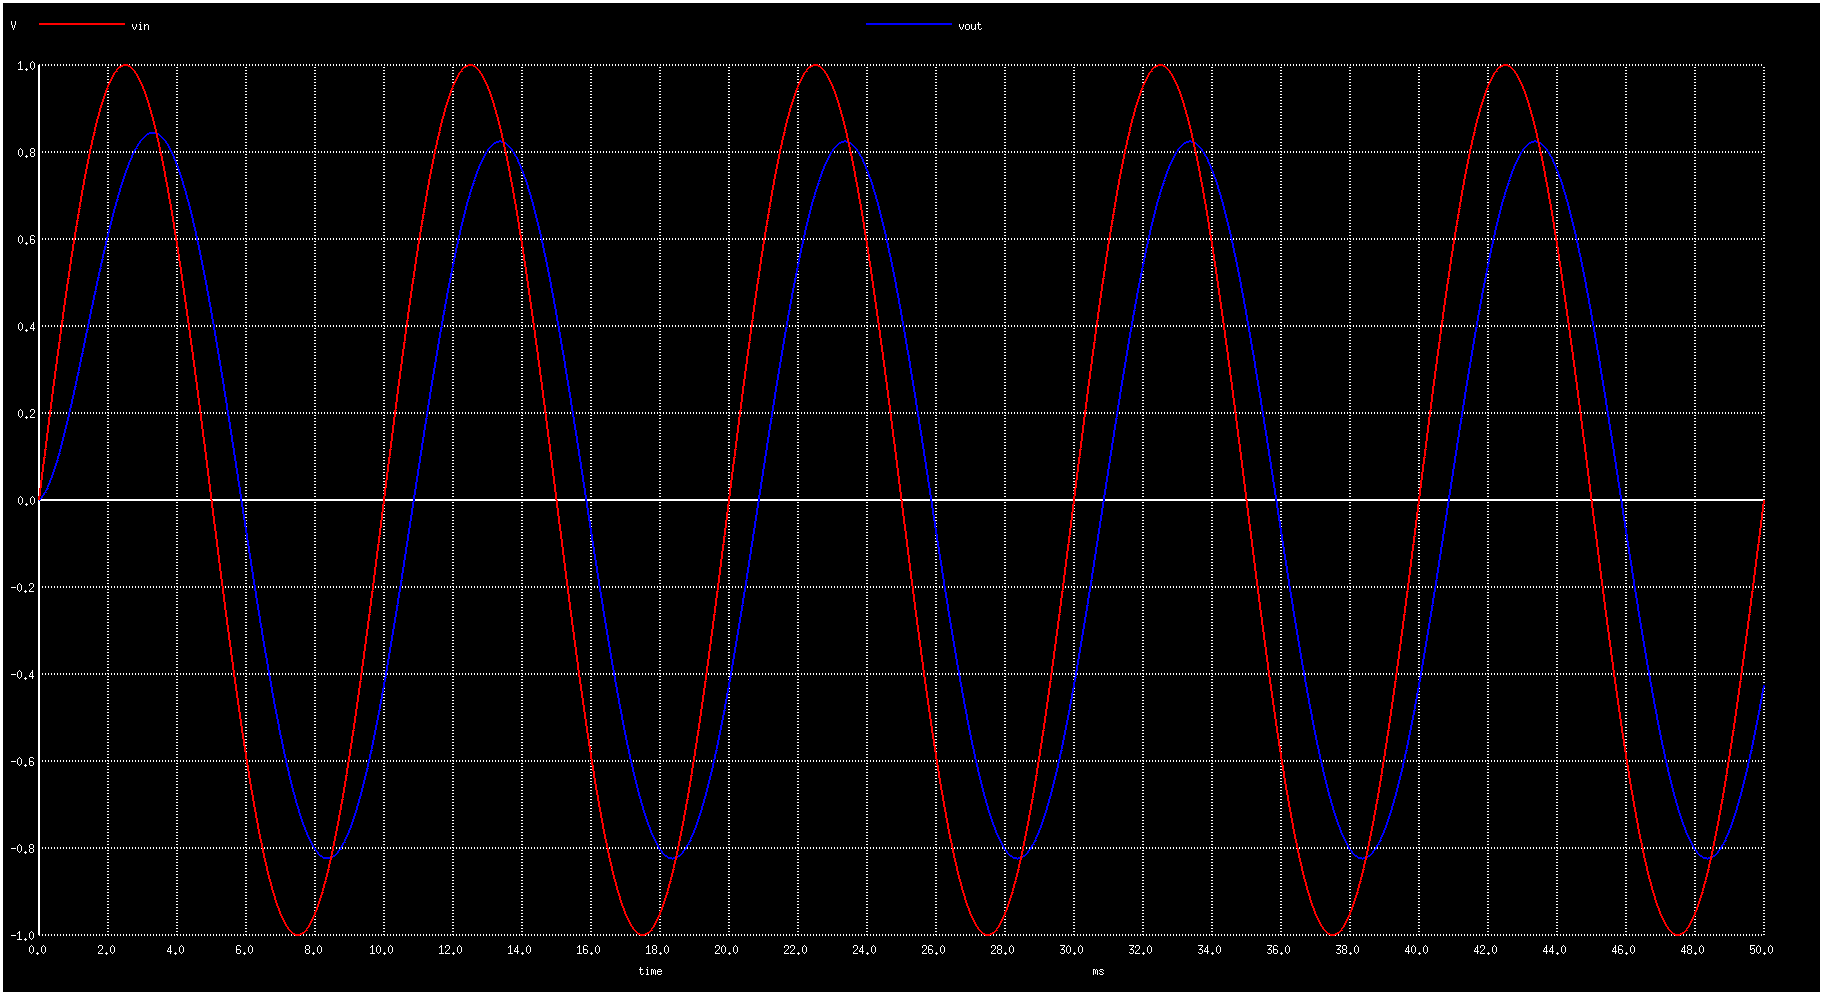
\includegraphics[scale=0.25]{Images/1b_1.png}
    \caption{$V_{out}$ and $V_{in}$ for $\omega = 2\pi \times 100 rad/sec$}
\end{figure}\\
Phase Lag at $\omega = 200\pi\times rad/sec$ is $-31.05^{\circ}$.

%Question-1b-2
\subsubsection{For $\omega_0 = 2\pi\times1M \text{ rad/sec}$}
\begin{lstlisting}
Question-1b_2

* Circuit
Vin	Vin	0	AC	1	SIN	0	1	1MEG
R	Vin	Vout	1k
C	Vout	1	1u
Rs	1	0	100

* Analysis
.tran 0.01n 5u

* Results
.control
run
plot Vin Vout
.endc

.end	
\end{lstlisting}

\textbf{Graph:}
\begin{figure}[!ht]
    \centering
    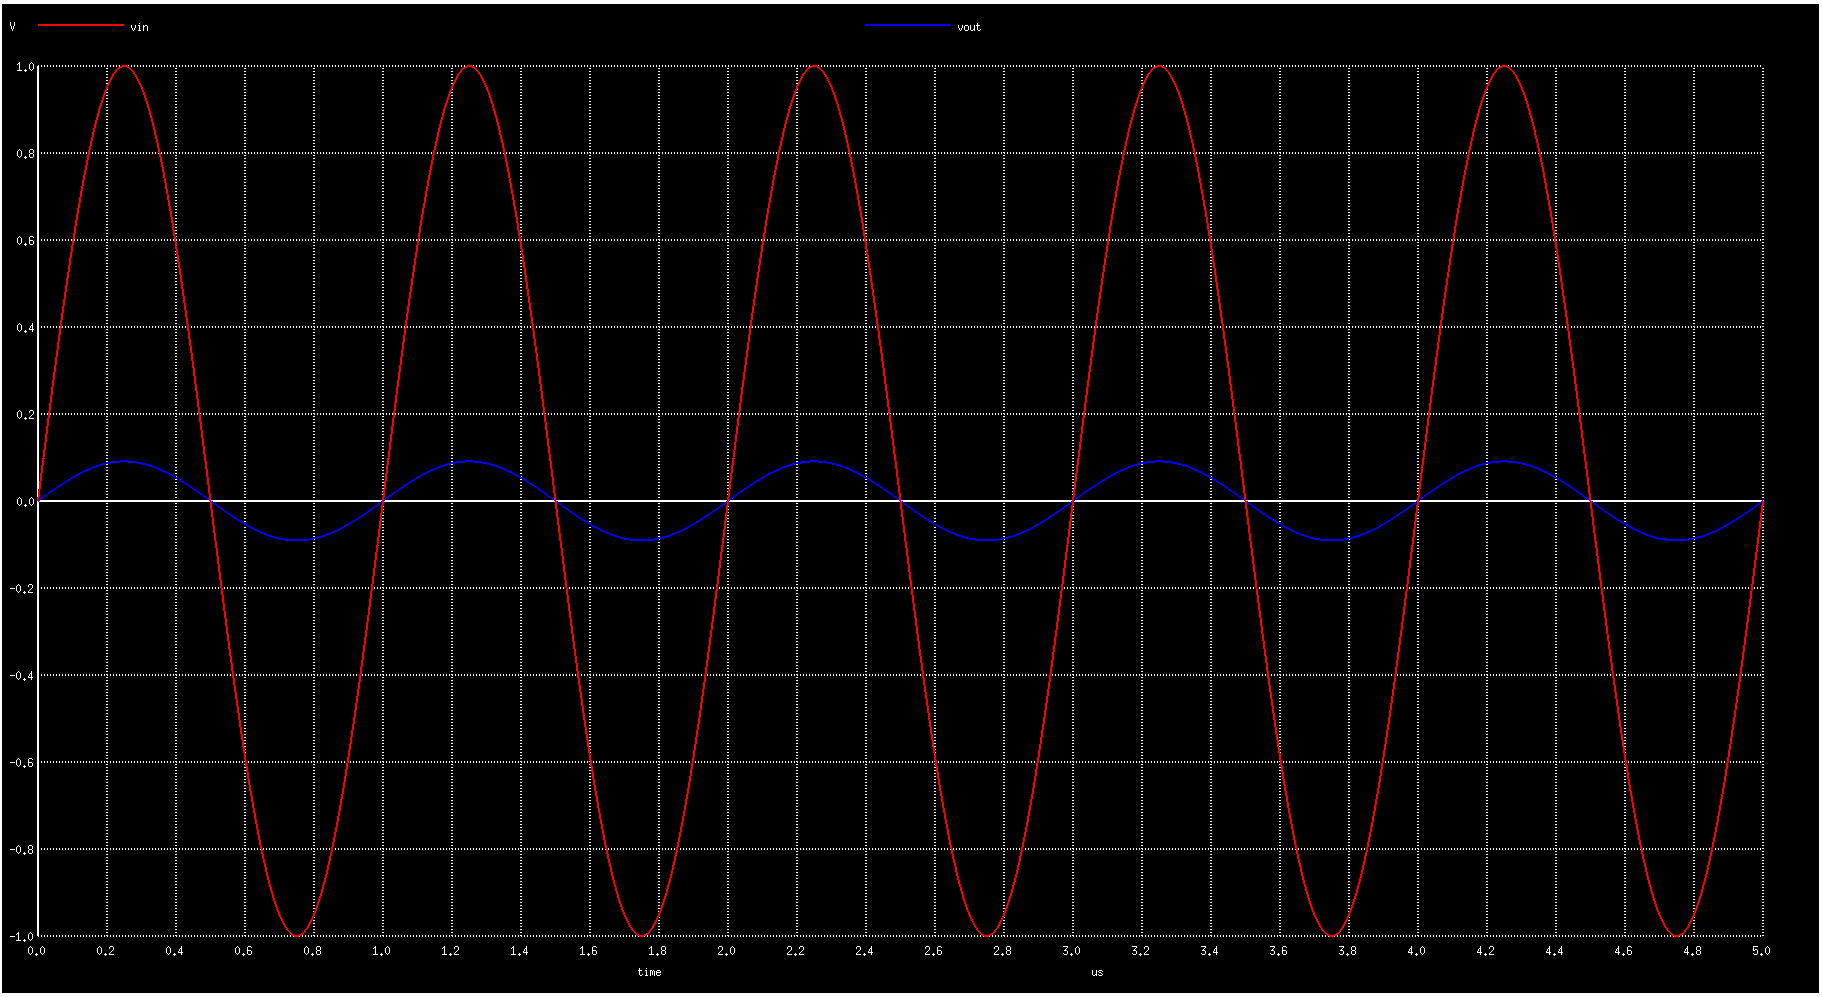
\includegraphics[scale=0.25]{Images/1b_2.png}
    \caption{$V_{out}$ and $V_{in}$ for $\omega = 2\pi\times\ 1M \text{ rad/sec}$}
\end{figure}\\
Phase Lag at $\omega = 2\pi\times10^6 rad/sec$ is $-0.9^{\circ} \approx 0^{\circ}$.
\\
These values can be verified by Phase - Transfer Characteristic in next sub-section.

% Question-1c
\subsection{1c}
For $V_{in} = \sin(\omega_0 t)$,\\
\begin{align}
    \frac{V_{\text {out}}}{V_{\text {in}}}=\frac{R_{S}Cj\omega_0+1}{C(R_{s}+R)j\omega_0+1} \\
    ||\frac{V_{\text {out}}}{V_{\text {in}}}|| = \sqrt{\left(\frac{1 + (CR_s\omega_0)^2}{1 + (C\omega_0(R+R_s))^2}\right)} \\
    \angle \frac{V_{out}}{V_{in}} = \tan ^{-1}\left({R_{s}C\omega_{0}}\right) - \tan ^{-1}\left({(R_{s} + R)C\omega_{0}}\right)
\end{align}\\
At 3dB point, $\frac{V_{out}}{V_{in}} = \frac{1}{\sqrt{2}}$. Frequency at 3dB point is $145.89 Hz$ and corresponding Phase is $-40^{\circ}$.\\
\textbf{SPICE Netlist:}
\begin{lstlisting}
Question-1c

* Circuit
Vin	Vin	0	AC	1	SIN	0	1	1000
R	Vin	Vout	1k
C	Vout	1	1u
Rs	1	0	100

* Analysis
.AC 	DEC 	10	1	1MEG

* Results
.control
run
plot db(Vout/Vin)
plot 180*(phase(Vout) - phase(Vin))/PI
.endc

.end
\end{lstlisting}
% Magnitude Plot
\textbf{Graph of Magnitude:}
\begin{figure}[!ht]
    \centering
    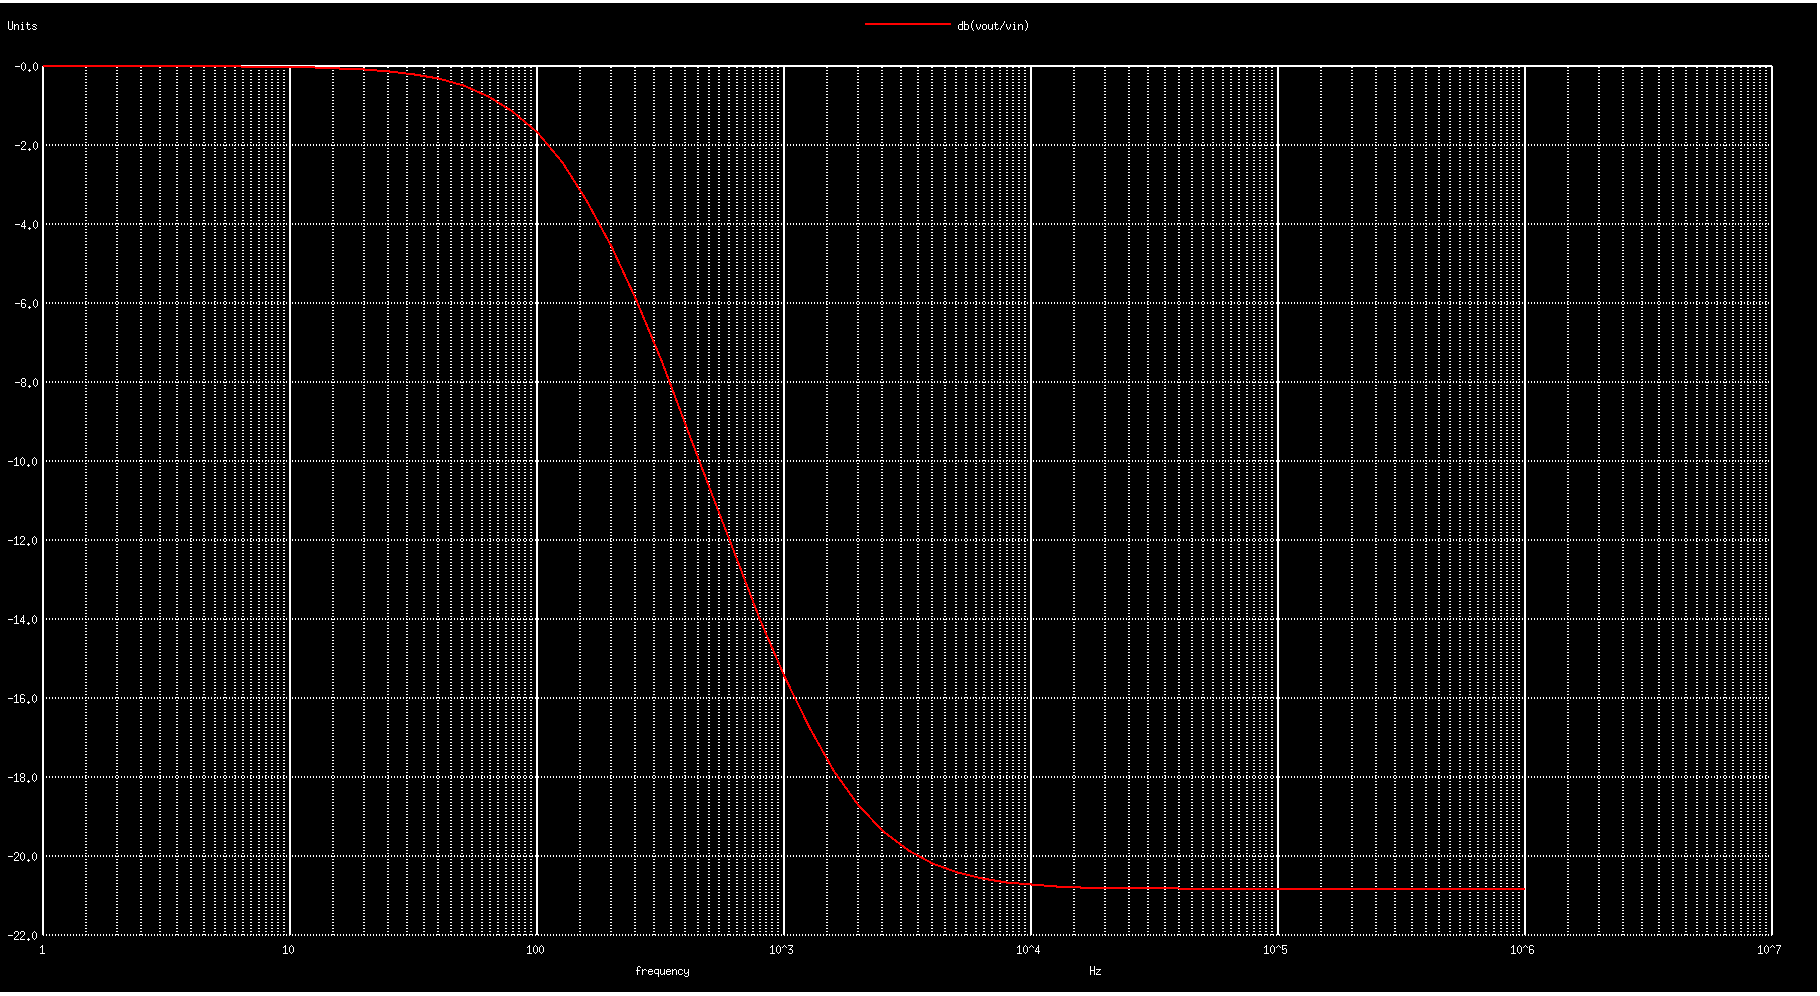
\includegraphics[scale=0.23]{Images/1c_1.png}
    \caption{$||\frac{V_{\text {out}}}{V_{\text {in}}}||$}
\end{figure}\\
% Phase Plot
\textbf{Graph of Phase:}
\begin{figure}[!ht]
    \centering
    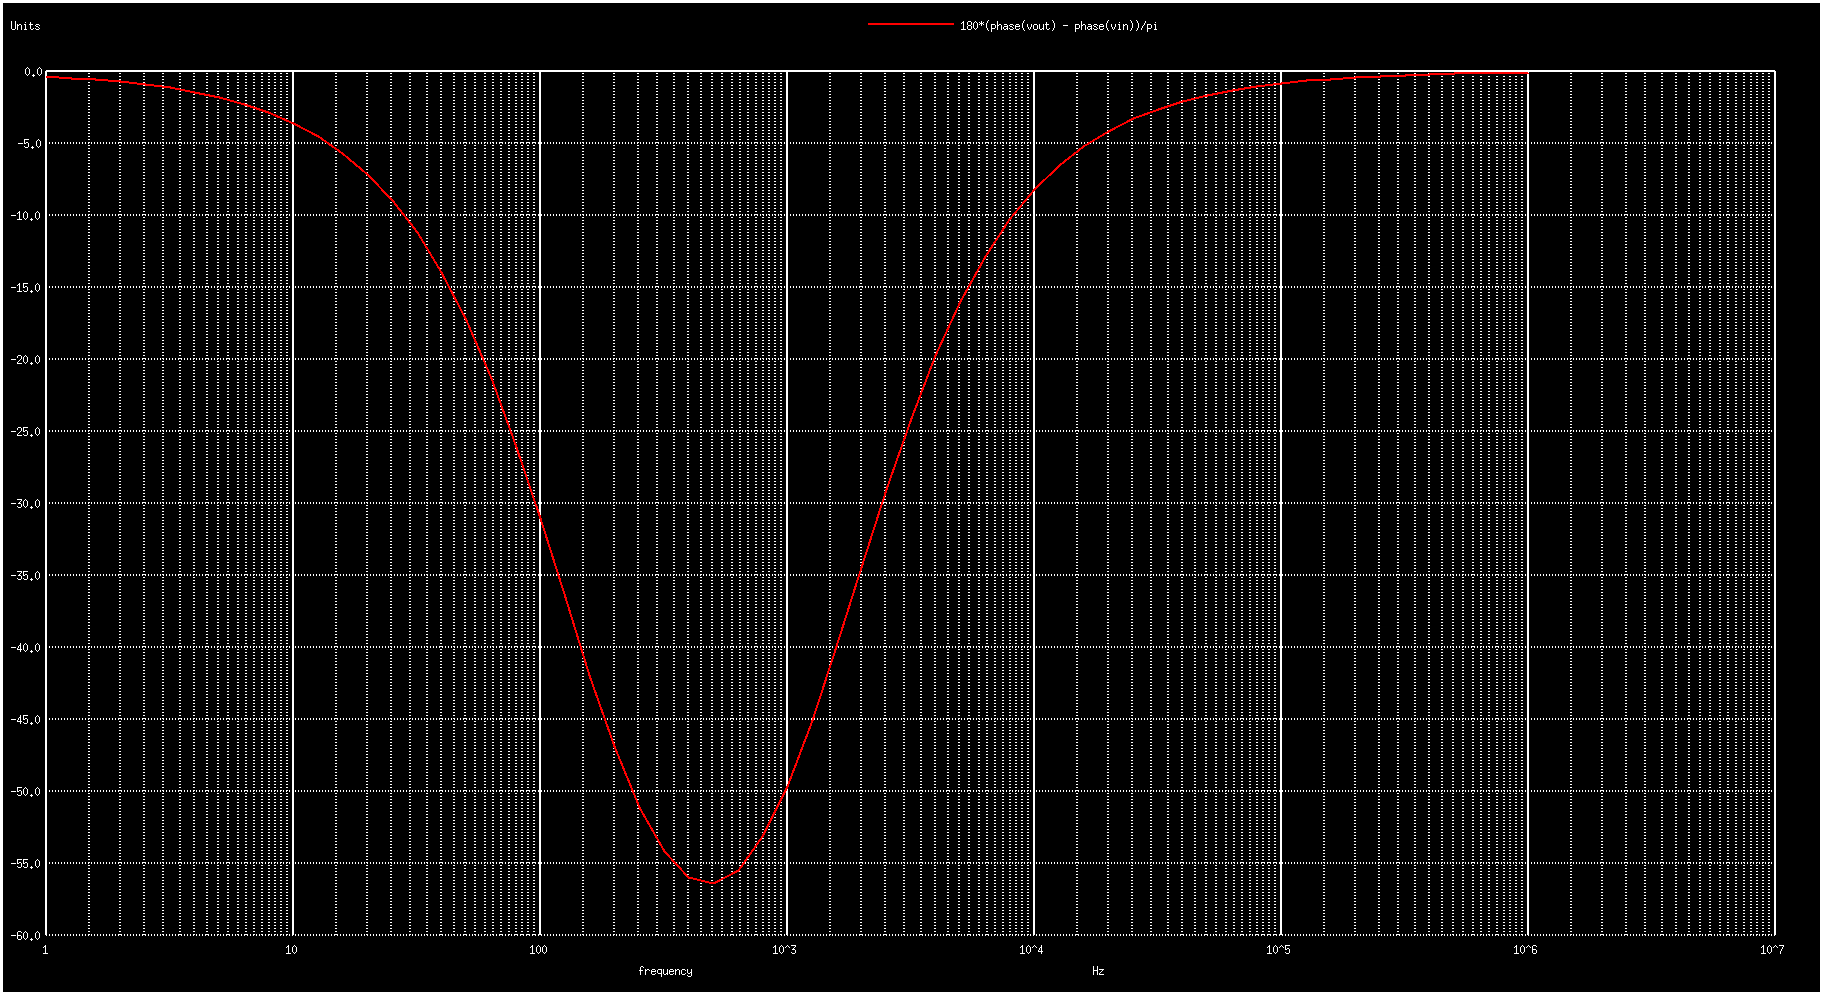
\includegraphics[scale=0.27]{Images/1c_2.png}
    \caption{$\angle \frac{V_{out}}{V_{in}}$}
\end{figure}\\

%% Question-2
\section{Analytic calculations vs SPICE simulations}
$I_s = 10^{-14} Amps$ and $T = 300K$ are standard conditions for a Ideal Diode. If we consider that $V_{Don} = 0.7 V$ for both Diodes, Current $i_D$ would be,
\begin{align}
    2.5 - 4\times10^3 i_D = 0.7 \times 2 \\
    i_D = \frac{1.1}{4000} = 2.75 \times 10^{-4} Amps
\end{align}
\begin{figure}[!ht]
    \centering
    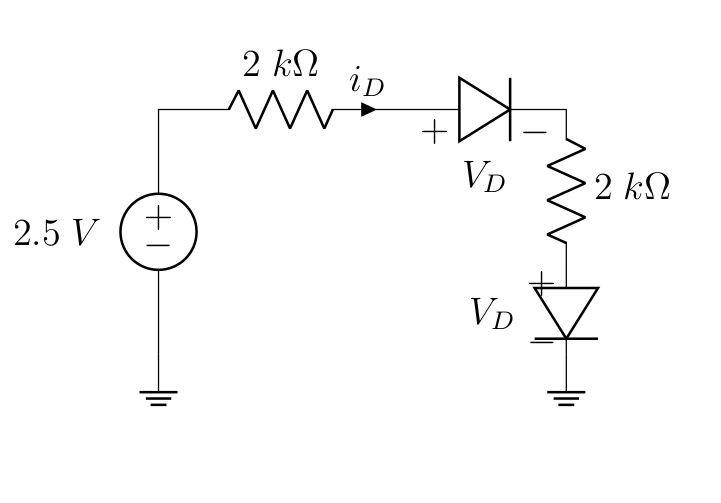
\includegraphics[scale=0.27]{Images/2.png}
\end{figure}
%Question-2c
\subsection{2c}
\textbf{SPICE Netlist:}
\begin{lstlisting}
Question-2c

* Circuit
V	Vin	0	DC	2.5
R1	Vin	1	2k
D1	1	Vout	CustomDiode
R2	Vout	2	2k
D2	2	0	CustomDiode

* Model
.model CustomDiode D

* Analysis
.op

* Results
.control
let ID = -Vin#branch
run
print all
.endc

.end
\end{lstlisting}
The results on Simulation are\\
\begin{align}
    V_D = 0.6250153 \text{ Volts}\\
    i_D = 3.12492 \times 10^{-4} \text{ Amps}    
\end{align}

%% Question-3
\section{Controlled Sources}
\begin{figure}[!ht]
    \centering
    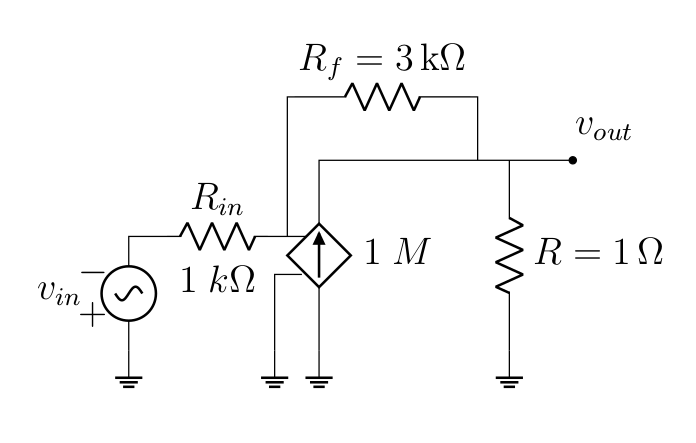
\includegraphics[scale=0.325]{Images/3.png}
\end{figure}\\
From the given properties,
\begin{align}
    V_{in} = 0.5\sin(2000\pi t)
\end{align}
And on solving using KCL and KVL and some valid approximations,
\begin{align}
    V_{out} = 3V_{in} \\
    V_{out} = 1.5\sin(2000\pi t)
\end{align}
\textbf{SPICE Netlist:}
\begin{lstlisting}
Question-3

* Circuit
Vin	0	1	AC	1	SIN	0	0.5	1k
Rin	1	2	1k
Rf	2	Vout	3k
R	Vout	0	1
G	Vout	0	2	0	1MEG

* Analysis
.tran 1u 0.005
*.AC 	DEC 	10	10	10MEG

* Results
.control
run
plot -V(1) V(Vout)
*plot -V(Vout)/V(1)
.endc

.end
\end{lstlisting}\\
\textbf{Graph:}
\begin{figure}[!ht]
    \centering
    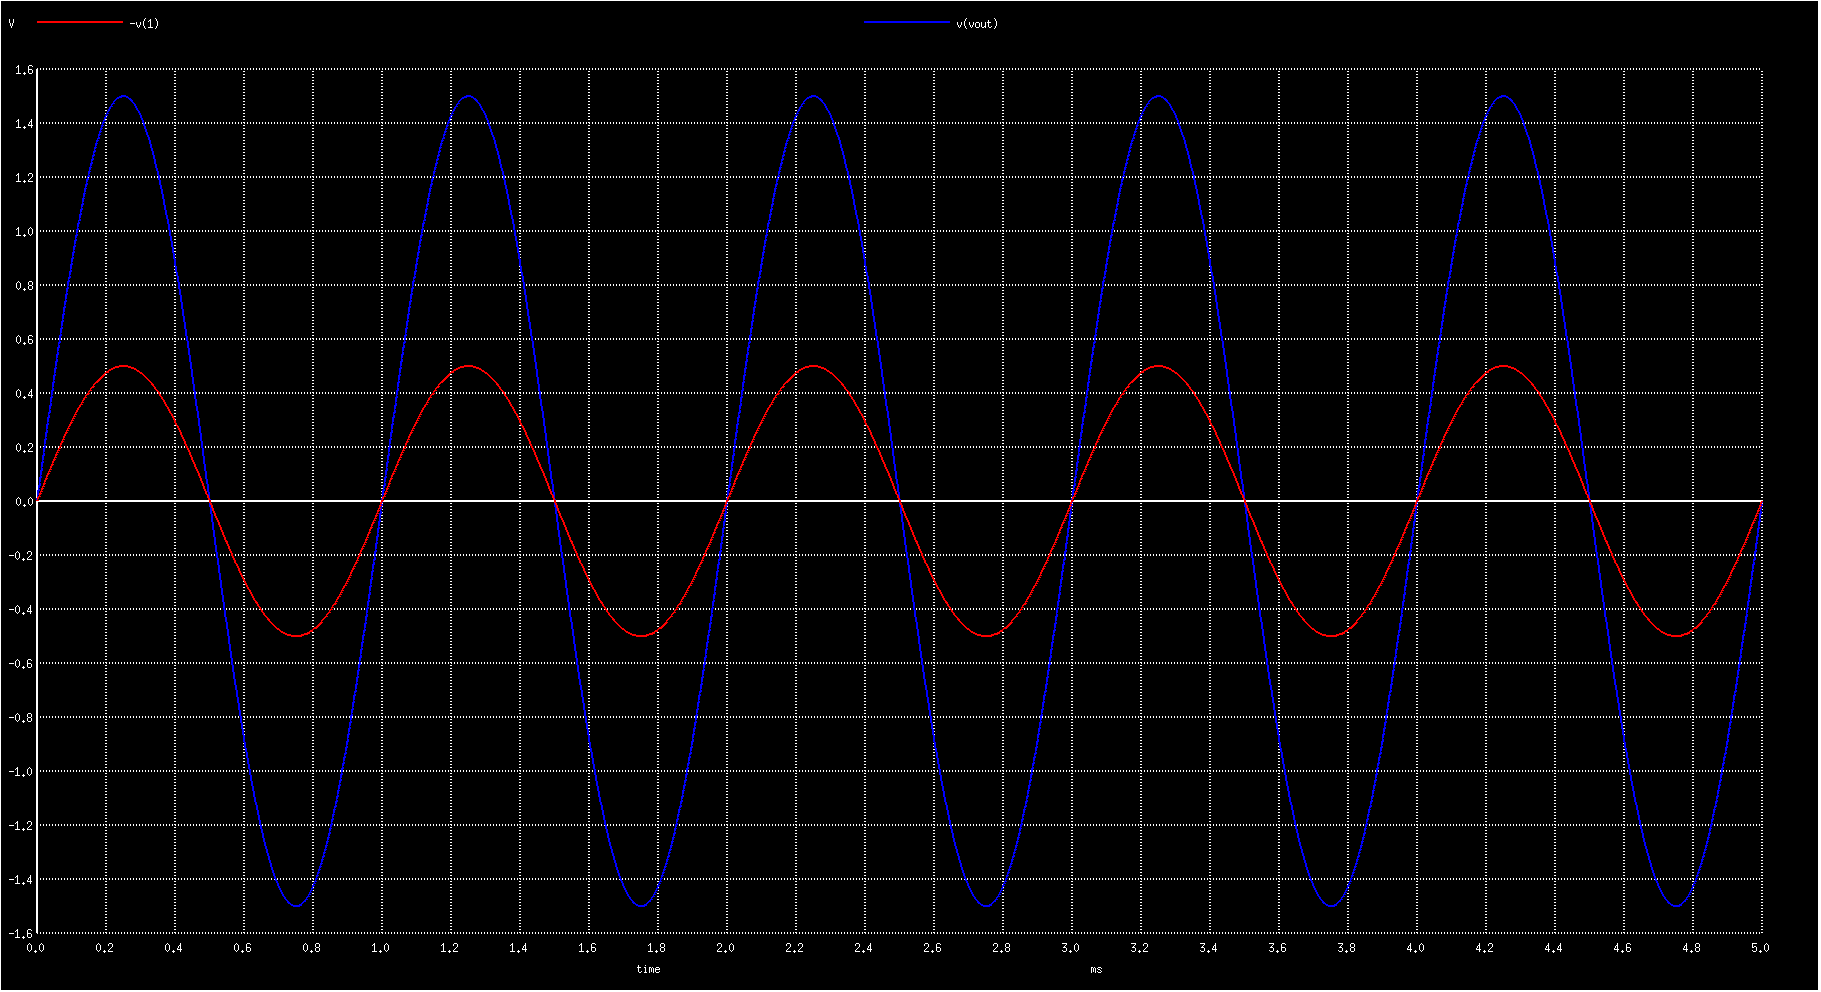
\includegraphics[scale=0.27]{Images/3_Graph.png}
    \caption{Plot of ${V_{out}}$ and ${V_{in}}$}
\end{figure}

%% Question-4
\section{MOSFET Characteristics}
\textbf{Long Channel MOSFET Parameters and Assumptions:}
\begin{enumerate}
    \item $\frac{W}{L}$ = 1.5
    \item L = 10$\mu$m
    \item W = 15$\mu$m
    \item $V_{GS}$ and $V_{DS}$ are supplied +ve.
\end{enumerate}
\\
\textbf{Short Channel MOSFET Parameters and Assumptions:}
\begin{enumerate}
    \item $\frac{W}{L}$ = 1.5
    \item L = 0.18$\mu$m
    \item W = 0.27$\mu$m
    \item $V_{GS}$ and $V_{DS}$ are supplied -ve.
\end{enumerate}
\\
\textbf{N-MOS Circuit:}
\begin{center}
    \begin{circuitikz}[american]
    \ctikzset{tripoles/mos style/arrows}
    \draw (0,1.5) node[nmos,](Q1){};
    \draw (Q1.center) node[right]{{$Q_{1}$}};
    \draw (0,0) node[ground](GND){} -- (Q1.S);
    \draw (Q1.G) to(-2,1.5) to[battery1, l= $V_{GS}$] (-2,0) node[ground](GND){};
    \draw (Q1.D) node[vcc](VCC){$V_{DS}$} (0,4.5);
    \end{circuitikz}
\end{center}

\textbf{P-MOS Circuit:}
\begin{center}
    \begin{circuitikz}[american]
    \ctikzset{tripoles/mos style/arrows}
    \draw (0,1.5) node[pmos,rotate=180,xscale=-1](Q1){};
    \draw (Q1.center) node[right]{{$Q_{1}$}};
    \draw (0,0) node[ground](GND){} -- (Q1.S);
    \draw (Q1.G) to(-2,1.5) to[battery1, l= $V_{GS}$] (-2,0) node[ground](GND){};
    \draw (Q1.D) node[vcc](VCC){$V_{DS}$} (0,4.5);
    \end{circuitikz}
\end{center}
% Question-4a
\subsection{4a}
\subsubsection{N-MOSFET}
\textbf{Long Channel SPICE Netlist:}
\begin{lstlisting}
Question-4anmosl
* Vgs value varies from 0.5,2 with a step of 0.5 *

* Circuit
M	td	tg	0	0	nch_tt	W = 15u L = 10u
Vgs	tg	0	DC	0.5
Vds	td	0	DC	0.5

* Model
.include "TSMC180.lib"
.model nch_tt nmos

* Analysis
.dc Vds 0 1.8 1m

* Results
.control
run
let ID = -Vds#branch
wrdata ../Data/4a/nmosl1.dat	V(td)	ID
plot ID vs V(td)
.endc

.end
\end{lstlisting}\\
\textbf{Short Channel SPICE Netlist:}
\begin{lstlisting}
Question-4anmoss
* Vgs value varies from 0.5,2 with a step of 0.5 *

* Circuit
M	td	tg	0	0	nch_tt	W = 0.27u L = 0.18u
Vgs	tg	0	DC	0.5
Vds	td	0	DC	0.5

* Model
.include "TSMC180.lib"
.model nch_tt nmos

* Analysis
.dc Vds 0 1.8 1m

* Results
.control
run
let ID = -Vds#branch
wrdata ../Data/4a/nmoss1.dat V(td) ID
plot ID vs V(td)
.endc

.end
\end{lstlisting}\\
\subsubsection{P-MOSFET}
\textbf{Long Channel SPICE Netlist:}
\begin{lstlisting}
Question-4apmosl
* Vgs value varies from -2,-0.5 with a step of 0.5 *

* Circuit
M	td	tg	0	0	pch_tt	W = 15u L = 10u
Vgs	tg	0	DC	-0.5
Vds	td	0	DC	-0.5

* Model
.include "TSMC180.lib"
.model pch_tt pmos

* Analysis
.dc Vds -1.8 0 1m

* Results
.control
run
let ID = -Vds#branch
wrdata ../Data/4a/pmosl1.dat	V(td)	ID
plot ID vs V(td)
.endc

.end
\end{lstlisting}\\
\textbf{Short Channel SPICE Netlist:}
\begin{lstlisting}
Question-4apmoss
* Vgs value varies from -2,-0.5 with a step of 0.5 *

* Circuit
M	td	tg	0	0	pch_tt	W = 0.27u L = 0.18u
Vgs	tg	0	DC	-0.5
Vds	td	0	DC	-0.5

* Model
.include "TSMC180.lib"
.model pch_tt pmos

* Analysis
.dc Vds -1.8 0 1m

* Results
.control
run
let ID = -Vds#branch
wrdata ../Data/4a/pmoss1.dat	V(td)	ID
plot ID vs V(td)
.endc

.end
\end{lstlisting}
\\
\subsubsection{Results}
\textbf{Python Code for Plotting Characteristics from Saved Data}
\begin{lstlisting}[language=Python]
#Python Code to Plot Simulation from Data

import numpy as np
import matplotlib.pyplot as plt

def File2Numpy(Path):
	Content = []
	for i in open(Path).readlines():
		Content.append(i.strip().split())
		
	Content = np.array(Content).astype(float)
	x = Content[:,1]
	y = Content[:,3]
	return np.array([x,y]).T
	
# Data of Long Channel N-MOSFET
ln1 = File2Numpy("../Data/4a/nmosl1.dat")
ln2 = File2Numpy("../Data/4a/nmosl2.dat")
ln3 = File2Numpy("../Data/4a/nmosl3.dat")
ln4 = File2Numpy("../Data/4a/nmosl4.dat")

# Data of Long Channel P-MOSFET
lp1 = File2Numpy("../Data/4a/pmosl1.dat")
lp2 = File2Numpy("../Data/4a/pmosl2.dat")
lp3 = File2Numpy("../Data/4a/pmosl3.dat")
lp4 = File2Numpy("../Data/4a/pmosl4.dat")

# Data of Short Channel N-MOSFET
sn1 = File2Numpy("../Data/4a/nmoss1.dat")
sn2 = File2Numpy("../Data/4a/nmoss2.dat")
sn3 = File2Numpy("../Data/4a/nmoss3.dat")
sn4 = File2Numpy("../Data/4a/nmoss4.dat")

# Data of Short Channel P-MOSFET
sp1 = File2Numpy("../Data/4a/pmoss1.dat")
sp2 = File2Numpy("../Data/4a/pmoss2.dat")
sp3 = File2Numpy("../Data/4a/pmoss3.dat")
sp4 = File2Numpy("../Data/4a/pmoss4.dat")


plt.figure(figsize=(20,20))

plt.subplot(2,2,1)
plt.plot(ln1[:,0],ln1[:,1],label=r"$V_{g}$ = 0.5")
plt.plot(ln2[:,0],ln2[:,1],label=r"$V_{g}$ = 1")
plt.plot(ln3[:,0],ln3[:,1],label=r"$V_{g}$ = 1.5")
plt.plot(ln4[:,0],ln4[:,1],label=r"$V_{g}$ = 2")
plt.title("Long Channel NMOS")
plt.grid()
plt.legend()
plt.xlabel(r"$V_{D}$")
plt.ylabel(r"$I_{D}$")

plt.subplot(2,2,2)
plt.plot(lp1[:,0],lp1[:,1],label=r"$V_{g}$ = -0.5")
plt.plot(lp2[:,0],lp2[:,1],label=r"$V_{g}$ = -1")
plt.plot(lp3[:,0],lp3[:,1],label=r"$V_{g}$ = -1.5")
plt.plot(lp4[:,0],lp4[:,1],label=r"$V_{g}$ = -2")
plt.title("Long Channel PMOS")
plt.grid()
plt.legend()
plt.xlabel(r"$V_{D}$")
plt.ylabel(r"$I_{D}$")

plt.subplot(2,2,3)
plt.plot(sn1[:,0],sn1[:,1],label=r"$V_{g}$ = 0.5")
plt.plot(sn2[:,0],sn2[:,1],label=r"$V_{g}$ = 1")
plt.plot(sn3[:,0],sn3[:,1],label=r"$V_{g}$ = 1.5")
plt.plot(sn4[:,0],sn4[:,1],label=r"$V_{g}$ = 2")
plt.title("Short Channel NMOS")
plt.grid()
plt.legend()
plt.xlabel(r"$V_{D}$")
plt.ylabel(r"$I_{D}$")

plt.subplot(2,2,4)
plt.plot(sp1[:,0],sp1[:,1],label=r"$V_{g}$ = -0.5")
plt.plot(sp2[:,0],sp2[:,1],label=r"$V_{g}$ = -1")
plt.plot(sp3[:,0],sp3[:,1],label=r"$V_{g}$ = -1.5")
plt.plot(sp4[:,0],sp4[:,1],label=r"$V_{g}$ = -2")
plt.title("Short Channel PMOS")
plt.grid()
plt.legend()
plt.xlabel(r"$V_{D}$")
plt.ylabel(r"$I_{D}$")

plt.savefig("4a.png")
plt.show()
\end{lstlisting}

\begin{figure}[!ht]
    \centering
    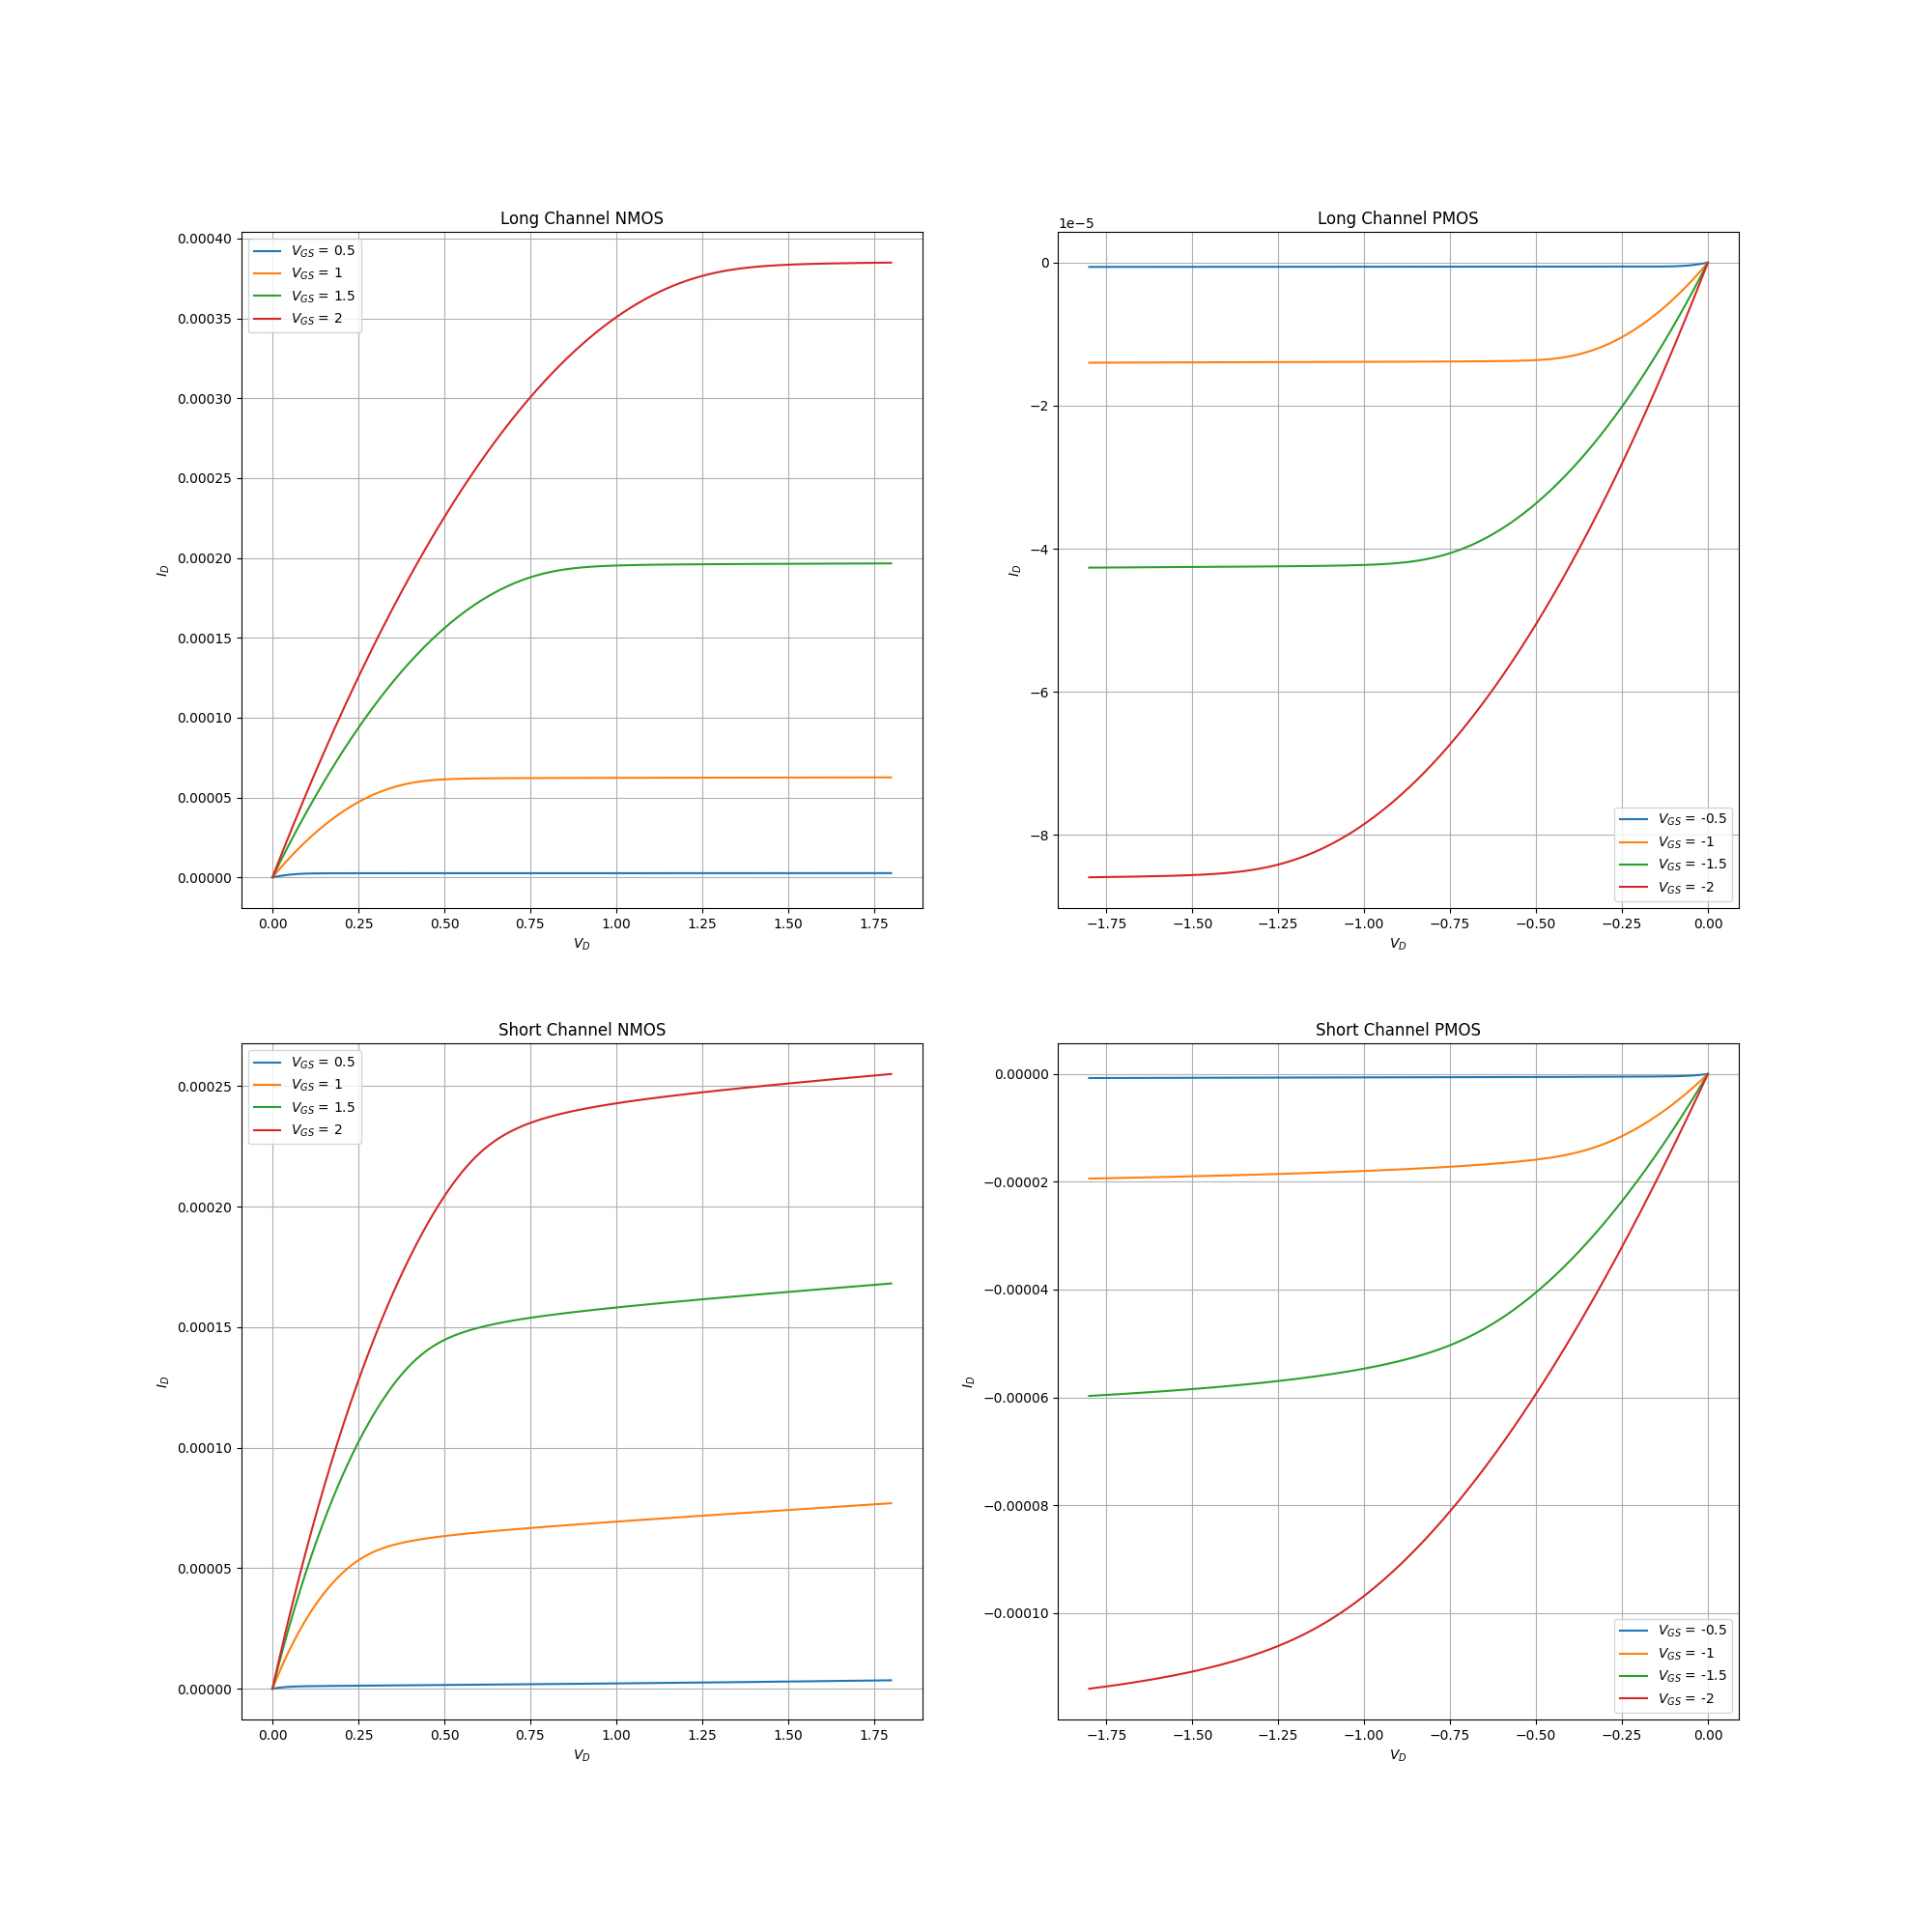
\includegraphics[scale=0.35]{Images/4a.png}
    \caption{$I_D$ vs $V_D$ Characteristics of Long and Short Channel N-MOSFETs and P-MOSFETs}
\end{figure}
% Question-4b
\subsection{4b}
\subsubsection{N-MOSFET}
\textbf{Long Channel SPICE Netlist:}
\begin{lstlisting}
Question-4bnmosl

* Circuit
M	td	tg	0	0	nch_tt	W = 15u L = 10u
Vgs	tg	0	DC	0.5
Vdd	td	0	DC	1.8

* Model
.include "TSMC180.lib"
.model nch_tt nmos

* Analysis
.dc Vgs 0 2 1m

* Results
.control
run
let ID = -Vdd#branch
wrdata ../Data/4b/nmosl.dat	V(tg)-0.362	ID
plot ID vs V(tg)-0.362
.endc

.end
\end{lstlisting}
\\
\textbf{Short Channel SPICE Netlist:}
\begin{lstlisting}
Question-4bnmoss

* Circuit
M	td	tg	0	0	nch_tt	W = 0.27u L = 0.18u
Vgs	tg	0	DC	0.5
Vdd	td	0	DC	1.8

* Model
.include "TSMC180.lib"
.model nch_tt nmos

* Analysis
.dc Vgs 0 2 1m

* Results
.control
run
let ID = -Vdd#branch
wrdata ../Data/4b/nmoss.dat	V(tg)-0.362	ID
plot ID vs V(tg)-0.362
.endc

.end
\end{lstlisting}
\subsubsection{P-MOSFET}
\textbf{Long Channel SPICE Netlist:}
\begin{lstlisting}
Question-4apmosl

* Circuit
M	td	tg	0	0	pch_tt	W = 15u L = 10u
Vgs	tg	0	DC	-0.5
Vdd	td	0	DC	-1.8

* Model
.include "TSMC180.lib"
.model pch_tt pmos

* Analysis
.dc Vgs -2 0 1m

* Results
.control
run
let ID = -Vdd#branch
wrdata ../Data/4b/pmosl.dat	V(tg)-0.388	ID
plot ID vs V(tg)-0.388
.endc

.end
\end{lstlisting}
\\
\textbf{Short Channel SPICE Netlist:}
\begin{lstlisting}
Question-4apmoss

* Circuit
M	td	tg	0	0	pch_tt	W = 0.27u L = 0.18u
Vgs	tg	0	DC	-0.5
Vdd	td	0	DC	-1.8

* Model
.include "TSMC180.lib"
.model pch_tt pmos

* Analysis
.dc Vgs -2 0 1m

* Results
.control
run
let ID = -Vdd#branch
wrdata ../Data/4b/pmoss.dat	V(tg)-0.388	ID
plot ID vs V(tg)-0.388
.endc

.end
\end{lstlisting}
\subsubsection{Results}
\textbf{Python Code for Plotting Characteristics from Saved Data}
\begin{lstlisting}[language=Python]
#Python Code to Plot Simulation from Data

import numpy as np
import matplotlib.pyplot as plt

def File2Numpy(Path):
	Content = []
	for i in open(Path).readlines():
		Content.append(i.strip().split())
		
	Content = np.array(Content).astype(float)
	x = Content[:,1]
	y = Content[:,3]
	return np.array([x,y]).T
	
# Data of Long Channel N-MOSFET
ln1 = File2Numpy("../Data/4a/nmosl1.dat")
ln2 = File2Numpy("../Data/4a/nmosl2.dat")
ln3 = File2Numpy("../Data/4a/nmosl3.dat")
ln4 = File2Numpy("../Data/4a/nmosl4.dat")

# Data of Long Channel P-MOSFET
lp1 = File2Numpy("../Data/4a/pmosl1.dat")
lp2 = File2Numpy("../Data/4a/pmosl2.dat")
lp3 = File2Numpy("../Data/4a/pmosl3.dat")
lp4 = File2Numpy("../Data/4a/pmosl4.dat")

# Data of Short Channel N-MOSFET
sn1 = File2Numpy("../Data/4a/nmoss1.dat")
sn2 = File2Numpy("../Data/4a/nmoss2.dat")
sn3 = File2Numpy("../Data/4a/nmoss3.dat")
sn4 = File2Numpy("../Data/4a/nmoss4.dat")

# Data of Short Channel P-MOSFET
sp1 = File2Numpy("../Data/4a/pmoss1.dat")
sp2 = File2Numpy("../Data/4a/pmoss2.dat")
sp3 = File2Numpy("../Data/4a/pmoss3.dat")
sp4 = File2Numpy("../Data/4a/pmoss4.dat")

# Transition
a = File2Numpy("../Data/4b/nmosl.dat")
b = File2Numpy("../Data/4b/pmosl.dat")
c = File2Numpy("../Data/4b/nmoss.dat")
d = File2Numpy("../Data/4b/pmoss.dat")

plt.figure(figsize=(20,20))

plt.subplot(2,2,1)
plt.plot(ln1[:,0],ln1[:,1],label=r"$V_{g}$ = 0.5")
plt.plot(ln2[:,0],ln2[:,1],label=r"$V_{g}$ = 1")
plt.plot(ln3[:,0],ln3[:,1],label=r"$V_{g}$ = 1.5")
plt.plot(ln4[:,0],ln4[:,1],label=r"$V_{g}$ = 2")
plt.plot(a[:,0],a[:,1],label=r"Transition")
plt.title("Long Channel NMOS")
plt.grid()
plt.legend()
plt.xlabel(r"$V_{D}$")
plt.ylabel(r"$I_{D}$")

plt.subplot(2,2,2)
plt.plot(lp1[:,0],lp1[:,1],label=r"$V_{g}$ = -0.5")
plt.plot(lp2[:,0],lp2[:,1],label=r"$V_{g}$ = -1")
plt.plot(lp3[:,0],lp3[:,1],label=r"$V_{g}$ = -1.5")
plt.plot(lp4[:,0],lp4[:,1],label=r"$V_{g}$ = -2")
plt.plot(b[:,0],b[:,1],label=r"Transition")
plt.title("Long Channel PMOS")
plt.grid()
plt.legend()
plt.xlabel(r"$V_{D}$")
plt.ylabel(r"$I_{D}$")

plt.subplot(2,2,3)
plt.plot(sn1[:,0],sn1[:,1],label=r"$V_{g}$ = 0.5")
plt.plot(sn2[:,0],sn2[:,1],label=r"$V_{g}$ = 1")
plt.plot(sn3[:,0],sn3[:,1],label=r"$V_{g}$ = 1.5")
plt.plot(sn4[:,0],sn4[:,1],label=r"$V_{g}$ = 2")
plt.plot(c[:,0],c[:,1],label=r"Transition")
plt.title("Short Channel NMOS")
plt.grid()
plt.legend()
plt.xlabel(r"$V_{D}$")
plt.ylabel(r"$I_{D}$")

plt.subplot(2,2,4)
plt.plot(sp1[:,0],sp1[:,1],label=r"$V_{g}$ = -0.5")
plt.plot(sp2[:,0],sp2[:,1],label=r"$V_{g}$ = -1")
plt.plot(sp3[:,0],sp3[:,1],label=r"$V_{g}$ = -1.5")
plt.plot(sp4[:,0],sp4[:,1],label=r"$V_{g}$ = -2")
plt.plot(d[:,0],d[:,1],label=r"Transition")
plt.title("Short Channel PMOS")
plt.grid()
plt.legend()
plt.xlabel(r"$V_{D}$")
plt.ylabel(r"$I_{D}$")

plt.savefig("4b.png")
plt.show()
\end{lstlisting}

\begin{figure}[!ht]
    \centering
    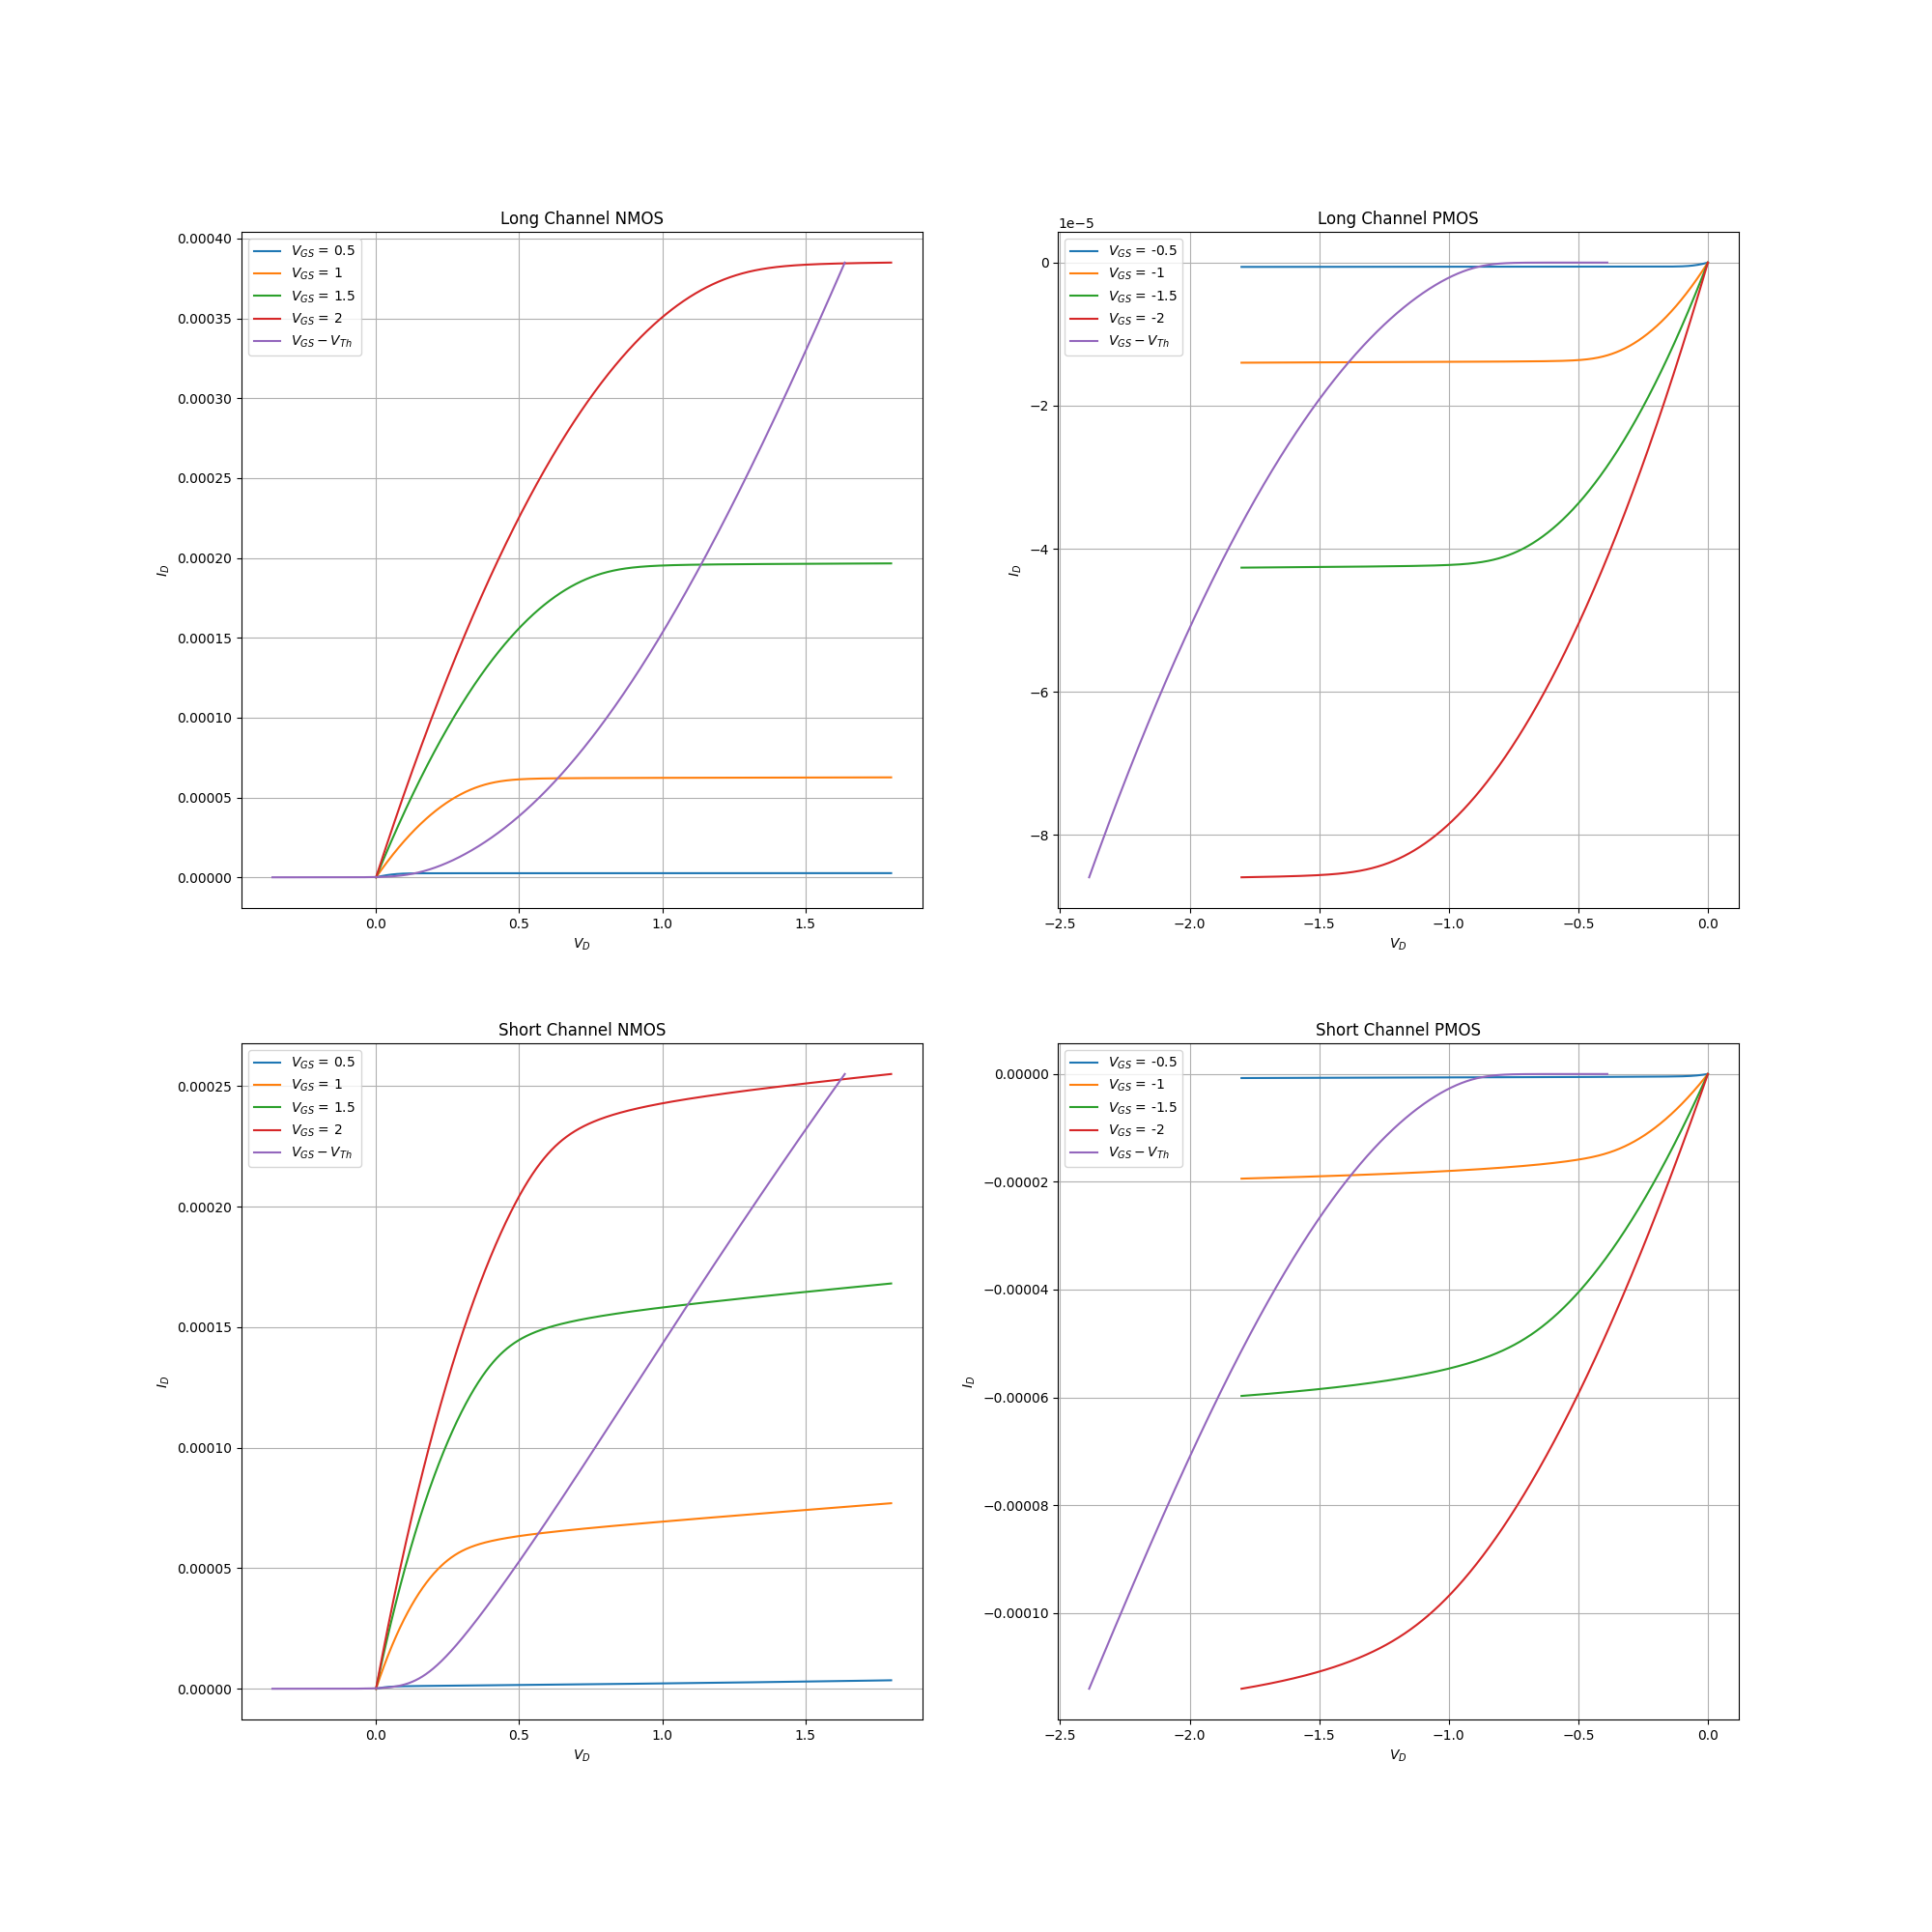
\includegraphics[scale=0.34]{Images/4b.png}
    \caption{$I_D$ vs $V_D$ Characteristics of Long and Short Channel N-MOSFETs and P-MOSFETs with Regions}
\end{figure}
The Graph of $I_D$ vs $V_{GS} - V_{Th}$ separates Linear Region from Saturation Region. The side of Parabolic Curve where $I_D$ vs $V_{D}$ varies Linearly is the Linear Region and the other one is Saturation Region.\\
\quad The Primary Difference between the Graphs in Long Channel and Short Channel MOSFETs is value of Channel Modulation Parameter $\lambda$. $\lambda \approx 0$ for Long Channel Devices and $\lambda$ is considerably large for Small Channel Devices. The considerable increase in $\lambda$ is one of the Short Channel Effects which happens due to shortening of length of the inverted channel region with increase in drain bias for large drain biases. For $\lambda = 0$, $I_D$ vs $V_{DS}$ graph saturates at the end whereas for considerable $\lambda$ $I_D$ vs $V_{DS}$ graph doesn't saturate.
% Question-4c
\subsection{4c}
The Small Signal Output Resistance $r_{0}$ parameter of the MOSFET doesn't depend on Small Signal Input Voltage. It also depends on Channel Modulation Parameter $\lambda$. It is independent on whether it is N-MOS or P-MOS.\\
\begin{align}
    g_{o}=\left.\frac{\partial i_{D}}{\partial v_{D S}}\right|_{Q}=\mu_{n} C_{o x}\left(\frac{W}{2 L}\right)\left(V_{G S}-V_{T n}\right)^{2} \lambda_{n} \cong \lambda I_{D} \\
    r_{o}=\frac{1}{g_{o}}=\frac{1}{\lambda I_{D}}
\end{align}
\subsubsection{Calculations}
Calculations are done for Graphs in Question-4a or for Section-4a in this document for $V_{GS} = 1.5$ Volts.
\begin{align}
    r_{0} = \frac{1}{(\frac{dI_D}{dV_{DS}})}\\
    r_{0} = \frac{dV_{DS}}{dI_D}
\end{align}
\textbf{N-MOSFET}\\
Long Channel Calculations:\\
\begin{align}
    \frac{dI_{D}}{dV_{DS}} = 0\\
    r_{0} \approx \infty
\end{align}
\\
Short Channel Calculations:\\
\begin{align}
    \frac{dI_{D}}{dV_{DS}} = 1.17647 \times 10^{-5} \text{ } \Omega^{-1}\\
    r_{0} = 85000 \text{ }\Omega
\end{align}
\textbf{P-MOSFET}\\
Long Channel Calculations:\\
\begin{align}
    \frac{dI_{D}}{dV_{DS}} = 2.117\times10^{-8} \text{ }\Omega^{-1}\\
    r_{0}  = 4.722 \times 10^7 \text{ }\Omega
\end{align}
\\
Short Channel Calculations:\\
\begin{align}
    \frac{dI_{D}}{dV_{DS}} = 1.468 \times 10^{-7} \text{ }\Omega^{-1}\\
    r_{0} = 6.8102 \times 10^6 \text{ }\Omega
\end{align}
\\
\pagebreak
%Question-4d
\subsection{4d}
\subsubsection{N-MOSFET}
\textbf{Long Channel}\\
SPICE Netlist:
\begin{lstlisting}
Question-4dnmosl

* Circuit
M	td	tg	0	0	nch_tt	W = 15u L = 10u
Vgs	tg	0	DC	0.5
Vdd	td	0	DC	1.8

* Model
.include "TSMC180.lib"
.model nch_tt nmos

* Analysis
.dc Vgs 0 2 0.1m

* Results
.control
run
let ID = -Vdd#branch
wrdata ../Data/4d/nmosl.dat	V(tg)	log10(ID)
plot log10(ID) vs V(tg)
.endc

.end
\end{lstlisting}\\
Plot:\\
\begin{figure}[!ht]
    \centering
    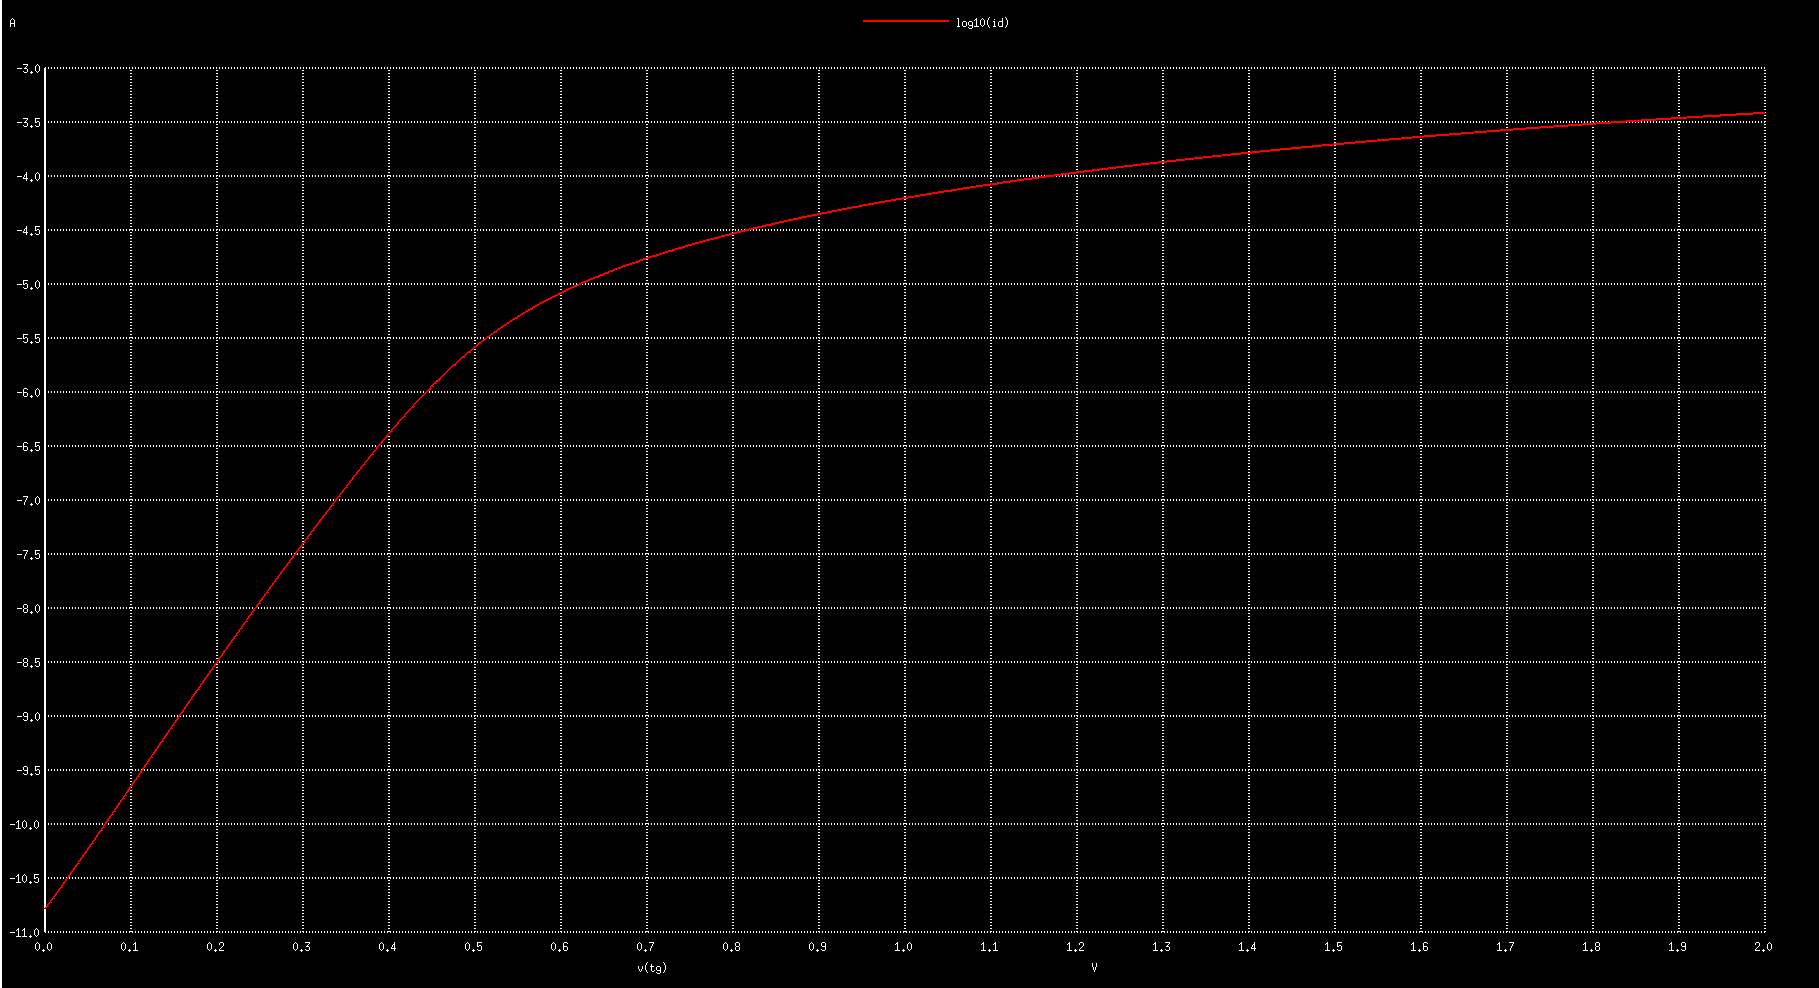
\includegraphics[scale=0.25]{Images/4dnmosl.png}
\end{figure}\\
Calculations:
\begin{align}
    S = 0.0921821 \text{ V/dec} \\
    S = \eta \frac{KT}{q} ln(10) \\
    \eta = 1.5514
\end{align}
\\
\textbf{Short Channel}\\
SPICE Netlist:
\begin{lstlisting}
Question-4dnmoss

* Circuit
M	td	tg	0	0	nch_tt	W = 0.27u L = 0.18u
Vgs	tg	0	DC	0.5
Vdd	td	0	DC	1.8

* Model
.include "TSMC180.lib"
.model nch_tt nmos

* Analysis
.dc Vgs 0 2 1m

* Results
.control
run
let ID = -Vdd#branch
wrdata ../Data/4d/nmoss.dat	V(tg)	log10(ID)
plot log10(ID) vs V(tg)
.endc

.end
\end{lstlisting}\\
Plot:\\
\begin{figure}[!ht]
    \centering
    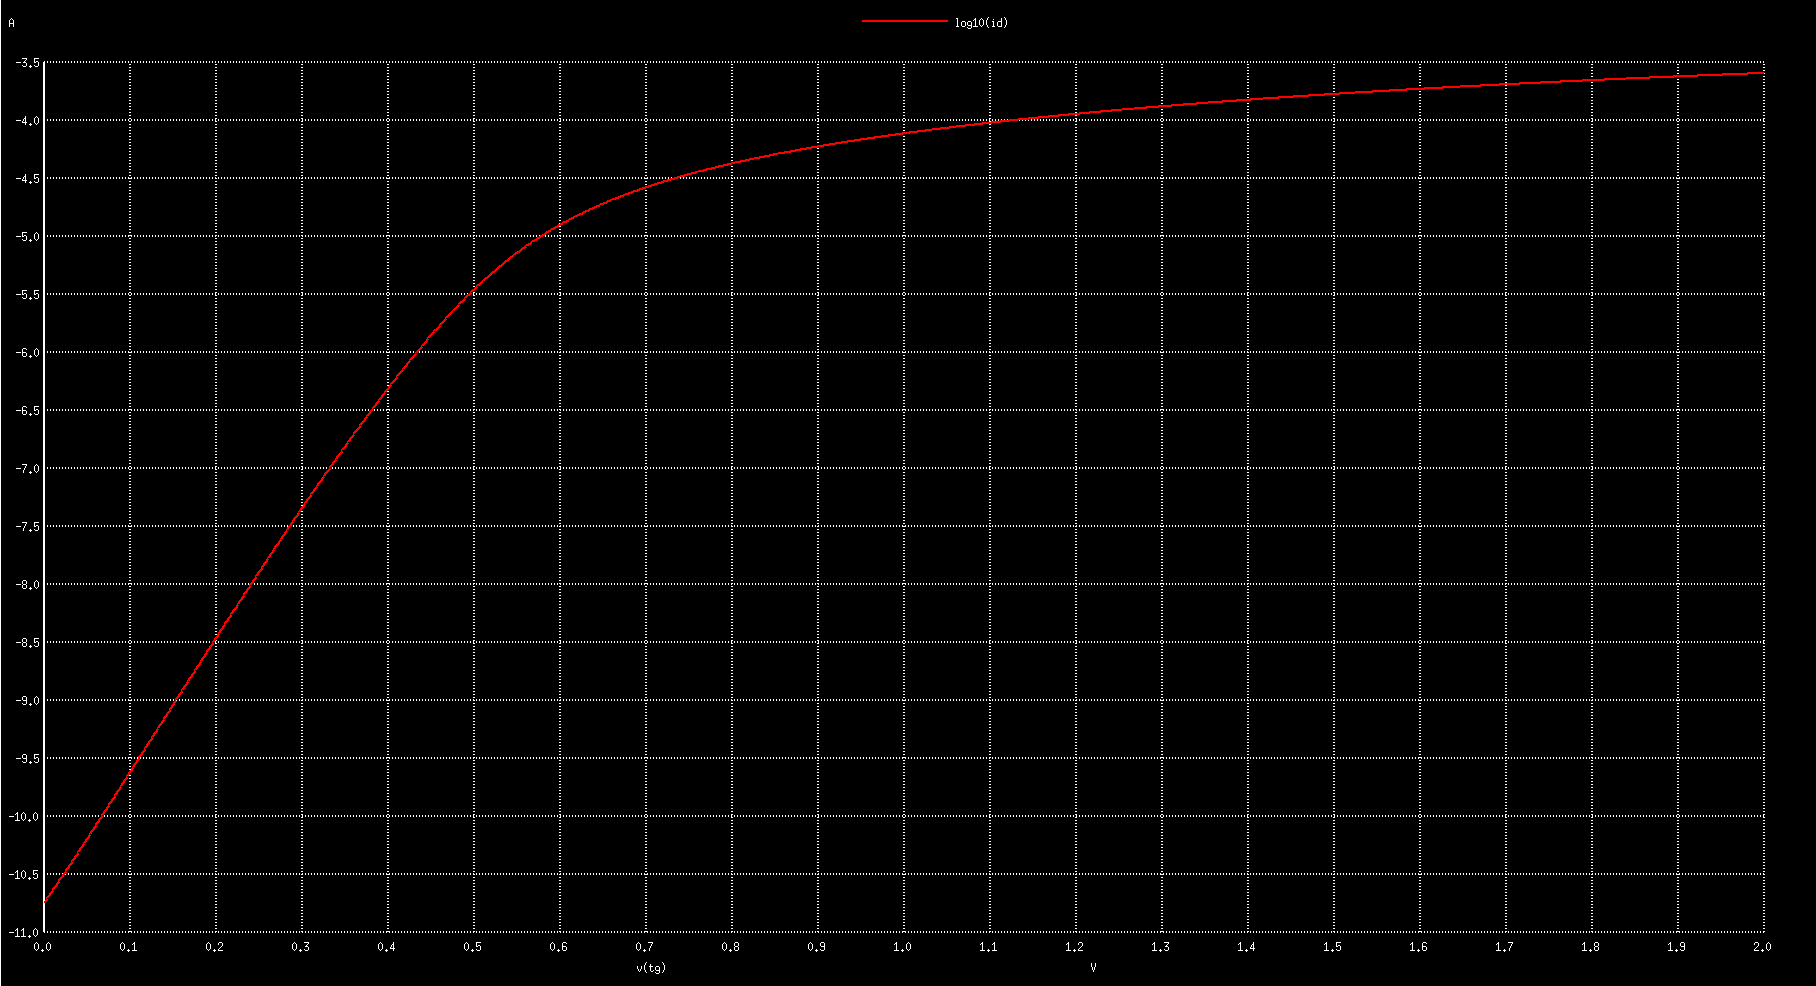
\includegraphics[scale=0.25]{Images/4dnmoss.png}
\end{figure}\\
Calculations:
\begin{align}
    S = 0.0906977 \text{ V/dec} \\
    S = \eta \frac{KT}{q} ln(10) \\
    \eta = 1.52645
\end{align}
\\
\subsubsection{P-MOSFET}
\textbf{Long Channel}\\
SPICE Netlist:
\begin{lstlisting}
Question-4dpmosl

* Circuit
M	td	tg	0	0	pch_tt	W = 15u L = 10u
Vgs	tg	0	DC	-0.5
Vdd	td	0	DC	-1.8

* Model
.include "TSMC180.lib"
.model pch_tt pmos

* Analysis
.dc Vgs -2 -0 1m

* Results
.control
run
let ID = -Vdd#branch
wrdata ../Data/4d/pmosl.dat	V(mag(tg))	log10(mag(ID))
plot log10(mag(ID)) vs mag(V(tg))
.endc

.end
\end{lstlisting}\\
Plot:\\
\begin{figure}[!ht]
    \centering
    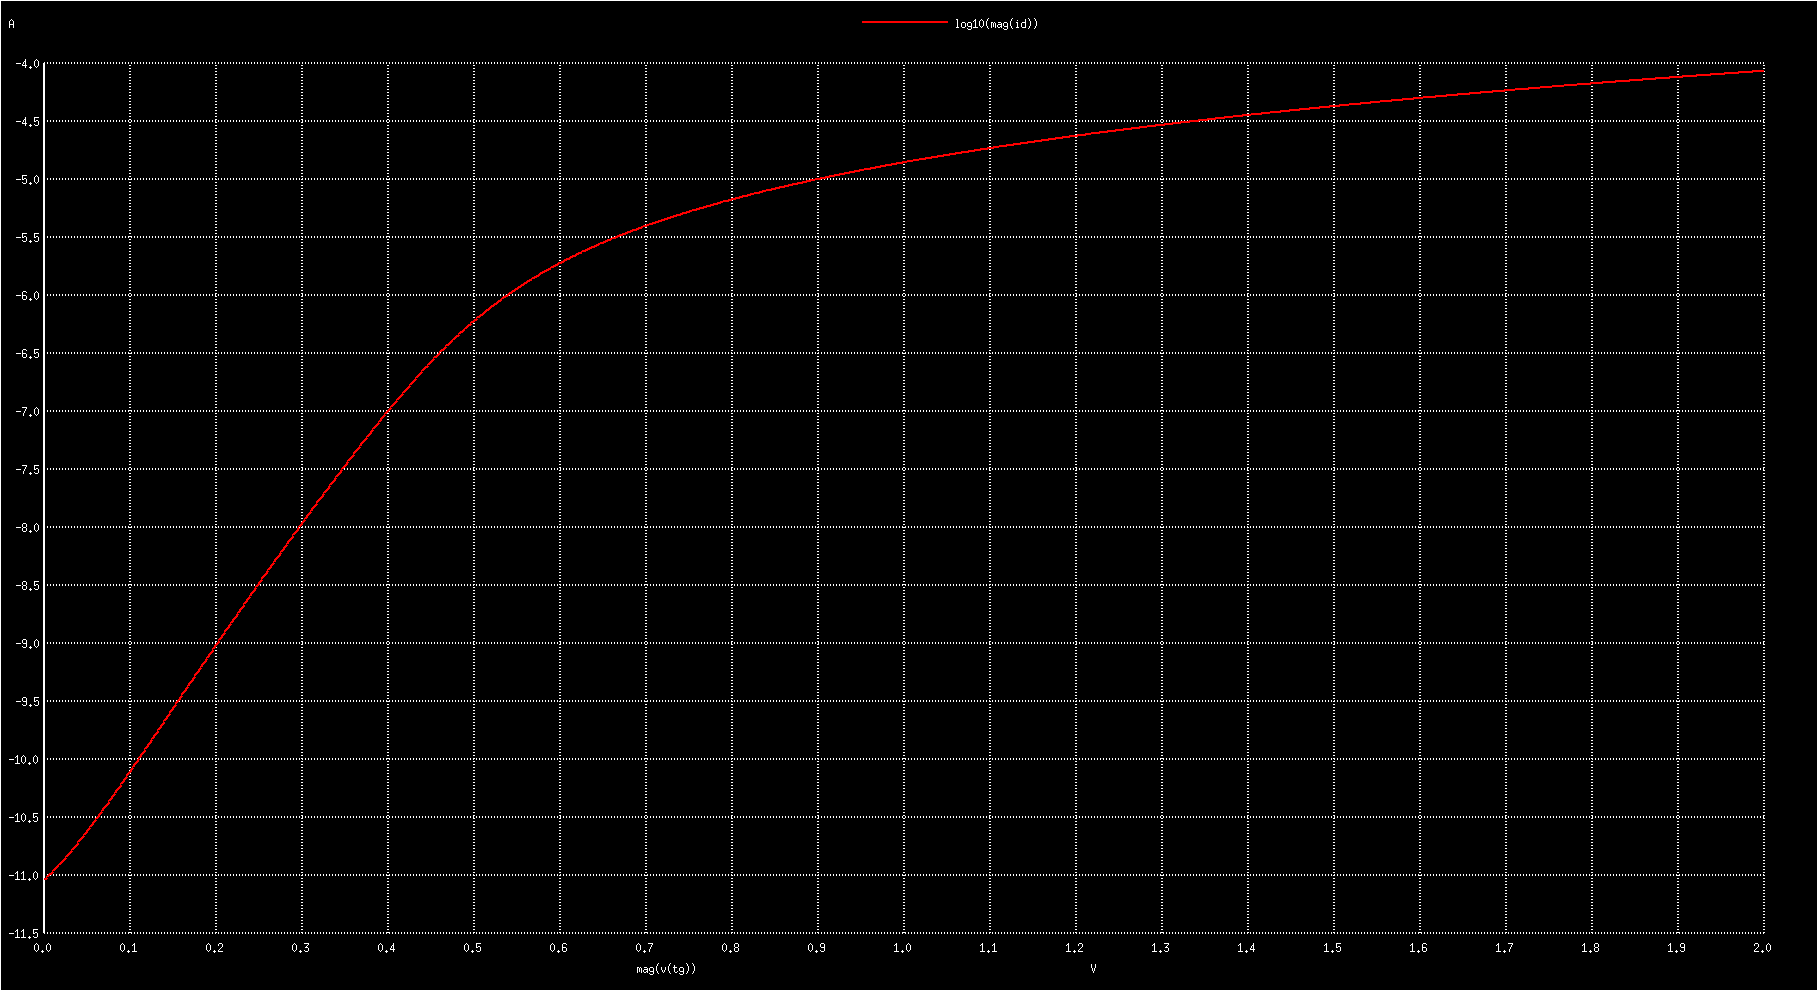
\includegraphics[scale=0.25]{Images/4dpmosl.png}
\end{figure}\\
Calculations:
\begin{align}
    S = 0.0930233 \text{ V/dec} \\
    S = \eta \frac{KT}{q} ln(10) \\
    \eta = 1.56559
\end{align}
\\
\textbf{Short Channel}\\
SPICE Netlist:
\begin{lstlisting}
Question-4dpmoss

* Circuit
M	td	tg	0	0	pch_tt	W = 0.27u L = 0.18u
Vgs	tg	0	DC	-0.5
Vdd	td	0	DC	-1.8

* Model
.include "TSMC180.lib"
.model pch_tt pmos

* Analysis
.dc Vgs -2 0 1m

* Results
.control
run
let ID = -Vdd#branch
wrdata ../Data/4d/pmoss.dat	mag(V(tg))	log10(mag(ID))
plot log10(mag(ID)) vs mag(V(tg))
.endc

.end
\end{lstlisting}\\
Plot:\\
\begin{figure}[!ht]
    \centering
    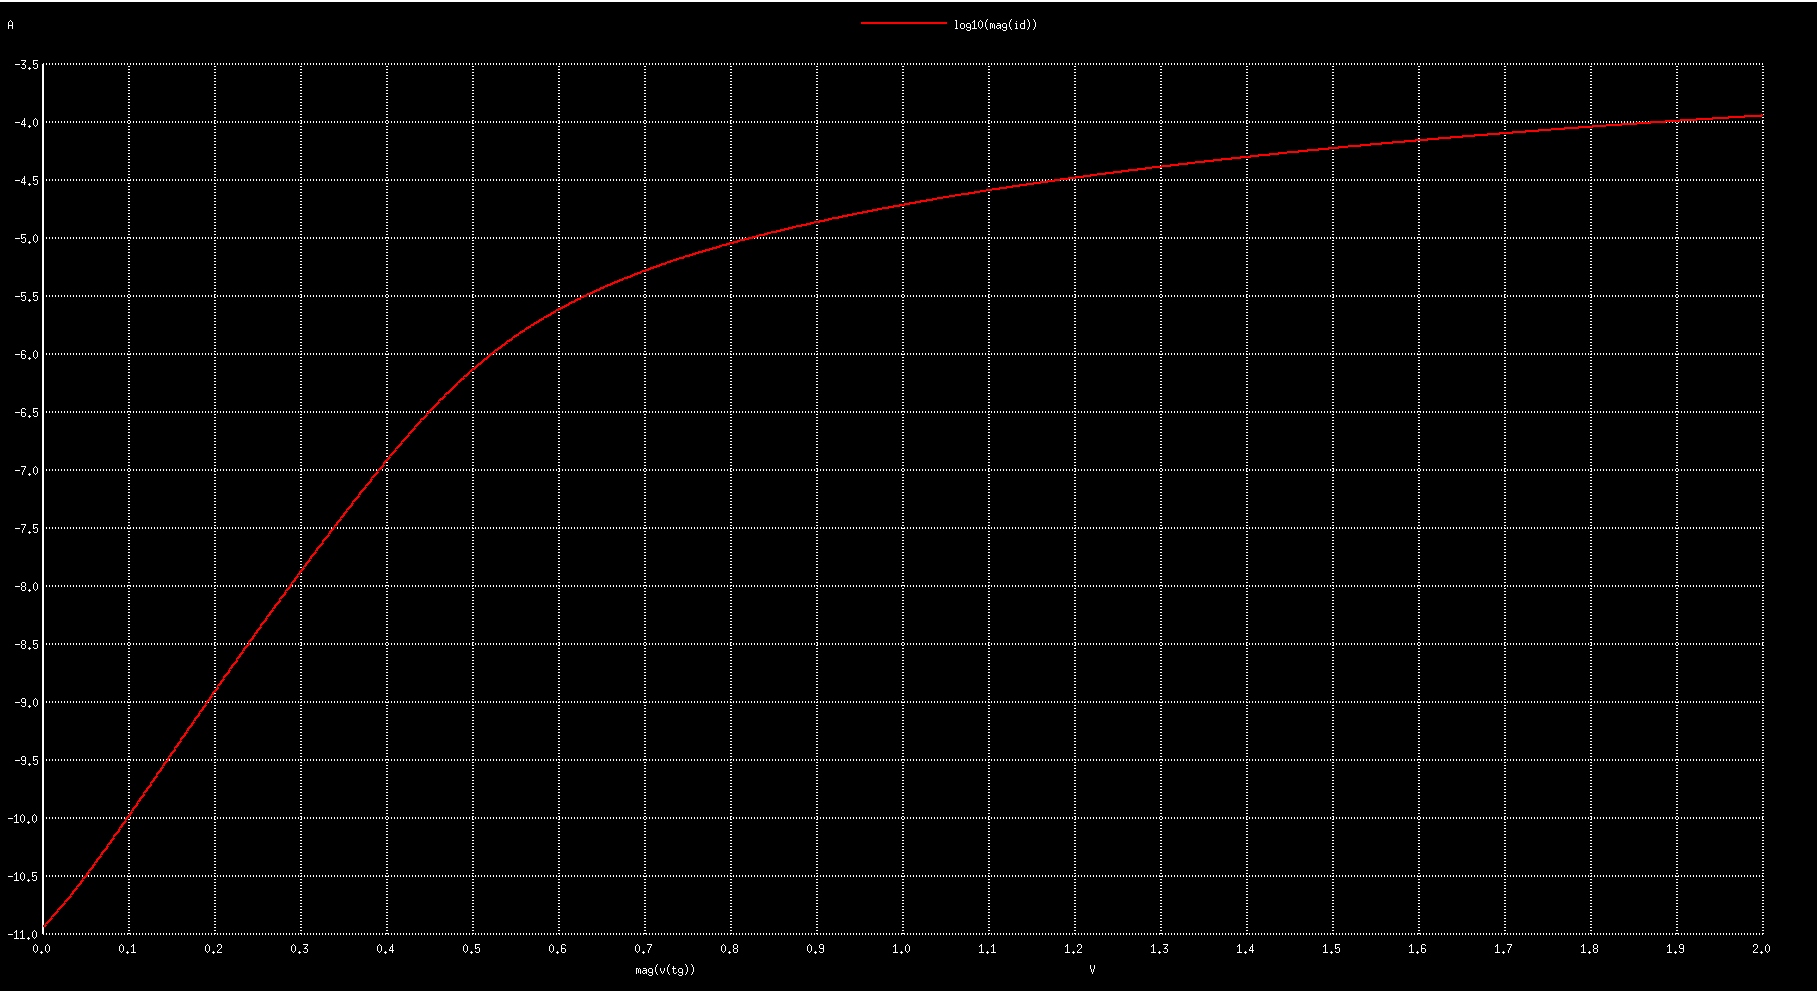
\includegraphics[scale=0.25]{Images/4dpmoss.png}
\end{figure}\\
Calculations:
\begin{align}
    S = 0.0991792 \text{ V/dec} \\
    S = \eta \frac{KT}{q} ln(10) \\
    \eta = 1.66919
\end{align}

%% Question-5
\section{Propagation Delay}
\textbf{Propagation Delay:} Propagation Delay is the difference between time taken by the Output to have its magnitude half of its Final Value and time taken for the Input to have its magnitude half of its Final Value.\\ 
\textbf{Rise Time:} Rise Time is the amount of time taken for the Signal to have its magnitude change from 10\% to 90\% of Steady State Value.\\
\begin{figure}[!ht]
    \centering
    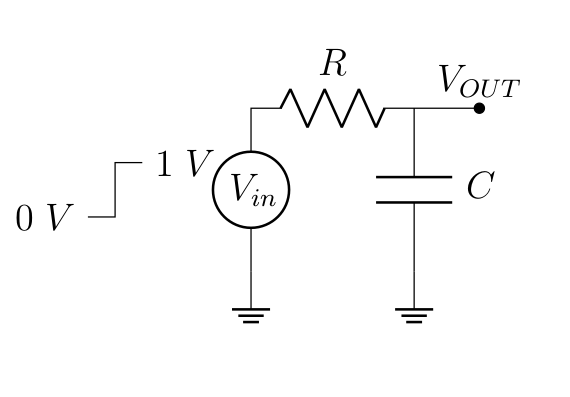
\includegraphics[scale=0.35]{Images/5.png}
\end{figure}
\subsection{5a}
When a Ideal Step Signal($t_{r,in} = 0$) is given as input to the given RC Circuit,
\begin{align}
    V_{out} = V_{in}(1 - e^{\frac{-t}{RC}})\\
    \text{Propagation Delay} = t_{p} = 0.69RC \\
    \text{Rise Time} = t_{r} = 2.2RC
\end{align}
Assuming,
\begin{align}
    R = 1000 \Omega\\
    C = 1\mu F \\
    t_{p} = 6.9 \times 10^{-4} s\\
    t_{r} = 2.2 \times 10^{-3} s
\end{align}
\textbf{SPICE Netlist:}
\begin{lstlisting}
*#destroy all

Vin	Vin	0	AC	1	PWL(0 0V   0 1V   1 1V)
R	Vin	Vout	1000
C	Vout	0	1u

* ANALYSIS
.tran 1u 0.008

* VIEW RESULTS
.control
run
plot Vin Vout
.endc

.end
\end{lstlisting}\\
\textbf{Graph:}
\begin{figure}[!ht]
    \centering
    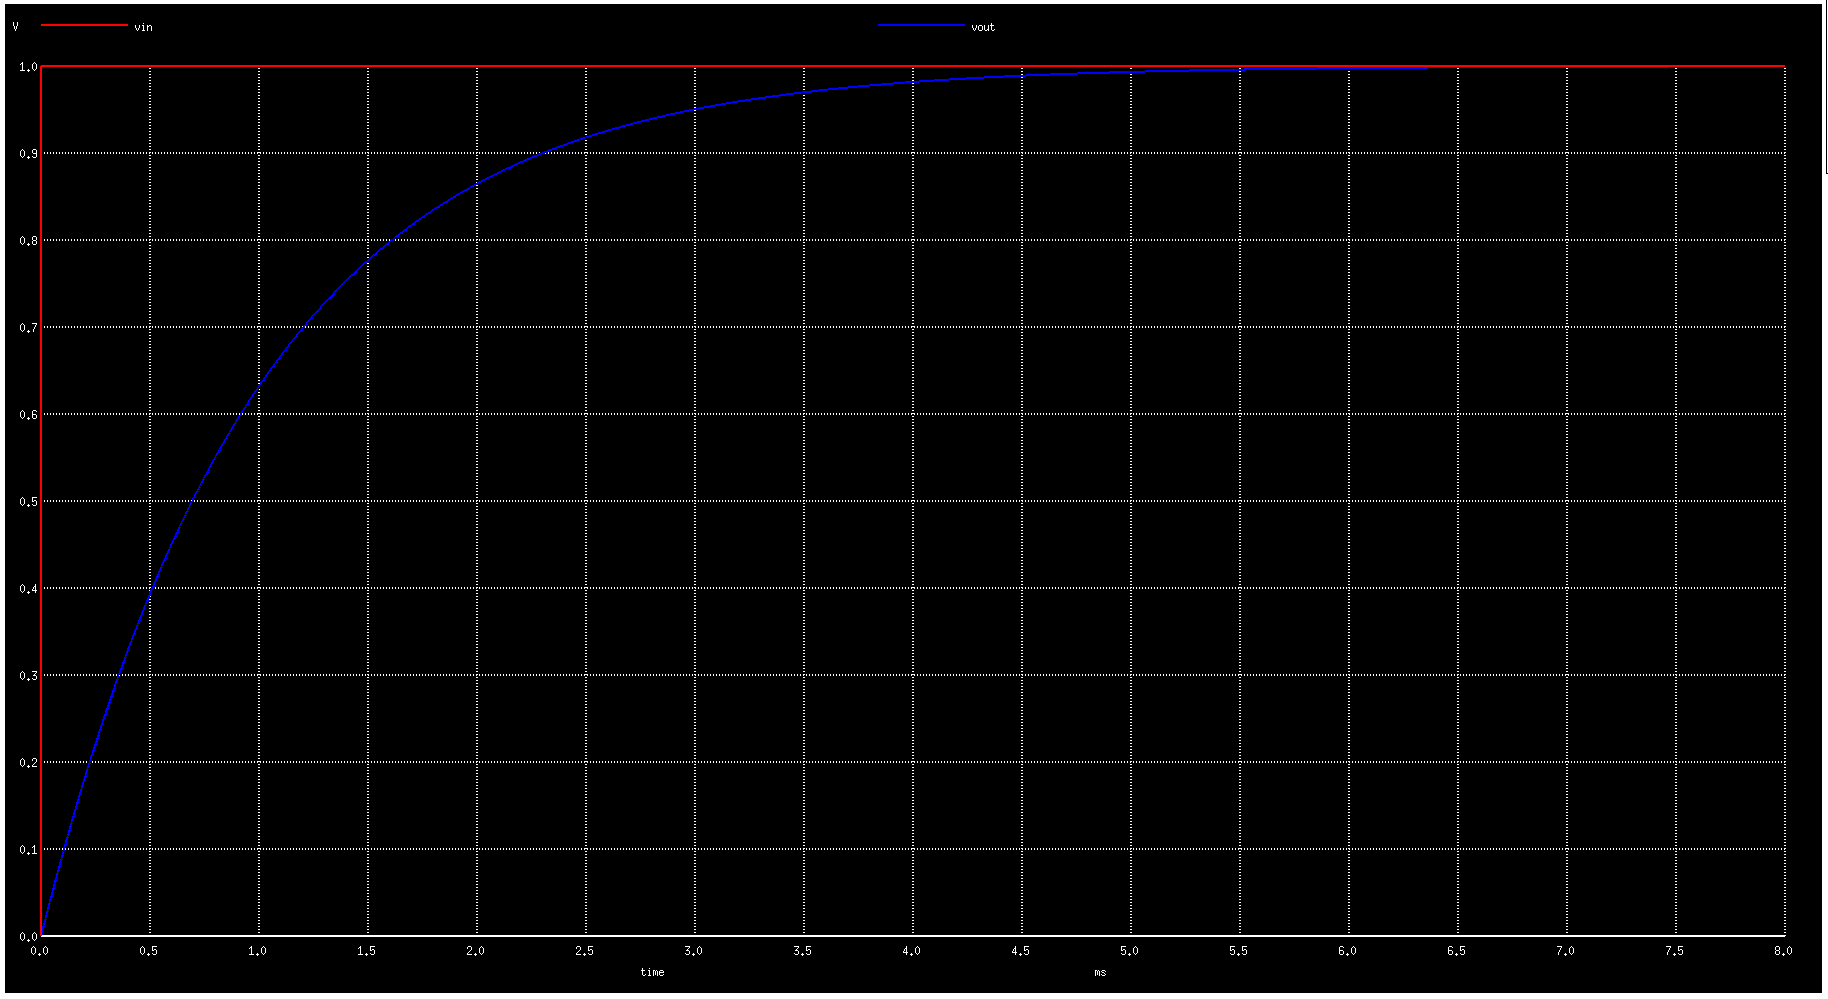
\includegraphics[scale=0.25]{Images/5a.png}
    \caption{$V_{out}$ and $V_{in}$ for Ideal Step Signal as Input}
\end{figure}

\subsection{5b}
\textbf{Parameters:}
\begin{align}
    R = 10 \Omega \\
    C = 1nF
\end{align}
\textbf{Readings:}
Table containing values of $\alpha = t_{r,in}/0.8$ and corresponding $t_{p,out}$.
\begin{center}
    \begin{tabular}{ |p{3cm}|p{3cm}| } 
    \hline
    $\alpha$ (in sec) & $t_{p,out}$ (in sec)\\ 
    \hline
    \hline
    10\times10^{-12} & 6.9434\times10^{-9}\\ 
    \hline
    50\times10^{-12} & 6.96226\times10^{-9}\\ 
    \hline
    100\times10^{-12} & 7\times10^{-9}\\ 
    \hline
    200\times10^{-12} & 7.02\times10^{-9}\\ 
    \hline
    300\times10^{-12} & 7.1\times10^{-9}\\
    \hline
    400\times10^{-12} & 7.137\times10^{-9}\\
    \hline
    500\times10^{-12} & 7.185\times10^{-9}\\
    \hline
    600\times10^{-12} & 7.23491\times10^{-9}\\
    \hline
    700\times10^{-12} & 7.28977\times10^{-9}\\
    \hline
    800\times10^{-12} & 7.34026\times10^{-9}\\
    \hline
    900\times10^{-12} & 7.39123\times10^{-9}\\
    \hline
    1\times10^{-9} & 7.44\times10^{-9}\\
    \hline
    2\times10^{-9} & 7.9\times10^{-9}\\
    \hline
    3\times10^{-9} & 8.47558\times10^{-9}\\
    \hline
    4\times10^{-9} & 9.00455\times10^{-9}\\
    \hline
    5\times10^{-9} & 9.54167\times10^{-9}\\
    \hline
    6\times10^{-9} & 1.00883\times10^{-8}\\
    \hline
    7\times10^{-9} & 1.06419\times10^{-8}\\
    \hline
    8\times10^{-9} & 1.12035\times10^{-8}\\
    \hline
    9\times10^{-9} & 1.17738\times10^{-8}\\
    \hline
    10\times10^{-9} & 1.23509\times10^{-8}\\
    \hline
    \end{tabular}
\end{center}
\begin{align}
    t_p = t_{p,out} - t_{p,in} \\
    t_{p,in} = \alpha/2
\end{align}
\textbf{Python Code for Simulation:}
\begin{lstlisting}[language=Python]
import numpy as np
import matplotlib.pyplot as plt

alpha = np.array([10*1e-12, 50*1e-12, 100*1e-12, 200*1e-12, 300*1e-12, 400*1e-12, 
		500*1e-12, 600*1e-12, 700*1e-12, 800*1e-12, 900*1e-12, 1*1e-9,
		2*1e-9, 3*1e-9, 4*1e-9, 5*1e-9, 6*1e-9, 7*1e-9, 8*1e-9, 9*1e-9, 10*1e-9])
		
tpout = np.array([6.9434*1e-9, 6.96226*1e-9, 7*1e-9, 7.02*1e-9, 7.1*1e-9, 7.137*1e-9,
        7.185*1e-9, 7.23491*1e-9, 7.28977*1e-9, 7.34026*1e-9, 7.39123*1e-9, 7.44*1e-9, 
        7.9*1e-9, 8.47558*1e-9, 9.00455*1e-9, 9.54167*1e-9, 1.008833*1e-8, 1.06419*1e-8, 
		1.12035*1e-8, 1.17738*1e-8, 1.23509*1e-8])

tr = 0.8*alpha
tpin = alpha/2
tp = tpout - tpin
		
plt.figure(figsize=(9,9))
plt.plot(tr,tp)
plt.grid()
plt.scatter(tr,tp)
plt.title(r"$t_{p}$ vs $t_{r,in}$")
plt.xlabel(r"$t_{r,in}$")
plt.ylabel(r"$t_{p}$")
plt.savefig("5b.png")
plt.show()
\end{lstlisting}
\textbf{Results:}
\begin{figure}[!ht]
    \centering
    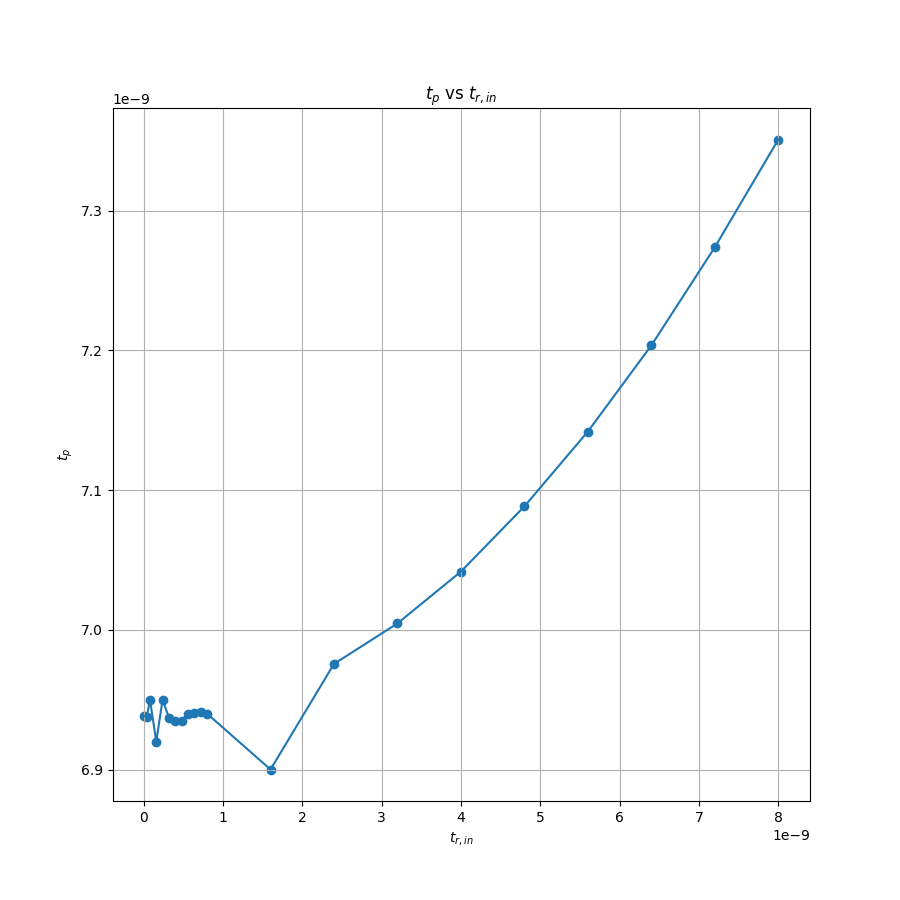
\includegraphics[scale=0.45]{Images/5b.png}
    \caption{Plot $t_{p}$ vs $t_{r,in}$}
\end{figure}
\end{document}